\documentclass{article}
\usepackage[english]{babel}
\usepackage[utf8x]{inputenc}
\usepackage[left=2cm,right=2cm,top=2cm,bottom=2cm]{geometry}
\usepackage{amssymb}
\usepackage{amsmath}
\usepackage{graphicx}
\usepackage[colorinlistoftodos]{todonotes}
\usepackage{hyperref}
\usepackage{float}
\usepackage{systeme}
\newcommand\tab[1][1cm]{\hspace*{#1}}
\usepackage{booktabs}
\usepackage{hyperref}
\newcommand{\tabitem}{~~\llap{\textbullet}~~}

\begin{document}
\begin{titlepage}
\newcommand{\HRule}{\rule{\linewidth}{0.1mm}} 
\center


\textsc{\Large Equation de Poisson et traitement d'image}\\[0.5cm]
\textsc{\Large Groupe de travail thématique}\\[0.5cm] 
\textsc{4TQMS801S}\\[0.5cm] 


\HRule \\[0.4cm]
{ \huge \bfseries Equation de Poisson et traitement d'image}\\[0.1cm] % Title of your Homework/assignment
\HRule \\[1.5cm]


\begin{minipage}{1.0\textwidth}
\Large  Virginie MONTALIBET \hfill Sébastien Eyzat 

\end{minipage}
\begin{minipage}{1.0\textwidth}
\end{minipage}\\[1cm]

{\Large \today}\\[1cm]

\includegraphics[width=15cm,  height=6cm,  keepaspectratio]
{Images/logo.png}
\vfill
\end{titlepage}
\newpage

\tableofcontents

\newpage
\section{Présentation du problème}
%%%%%%%%%%%%%%%%%%%%%%%%%%%%%%%%%%%%%%%%%%%%%%%%%%%%%%%%%%%
%                       EXPOSITION DU SUJET               %
%%%%%%%%%%%%%%%%%%%%%%%%%%%%%%%%%%%%%%%%%%%%%%%%%%%%%%%%%%%

Le traitement d'images est un ensemble de méthodes permettant d'étudier et de transformer une ou plusieurs images à l'aide de moyens mathématiques et numériques. Le principe du traitement d'images consiste à extraire certaines informations de celles-ci, afin de les étudier ou de les modifier.Il est utilisé dans beaucoup d'applications telles que l'amélioration du contraste, l'application d'un filtre(flou, lissage, changement de couleurs), ou encore les détections et identifications d'objets par exemple. 

Dans ce rapport, nous nous intéresserons à l'incrustation d'images. À partir de deux images, comment sélectionner une partie de la première et l'incruster de la manière la plus naturelle possible dans la seconde ? 
\newline
Afin d'éclaircir nos propos et d'identifier les problèmes que nous devons résoudre, voici un exemple de ce que nous souhaitons faire.\newline
Nous disposons des deux images présentées ci-dessous, l'image T(arget) et l'image S(ource). 
\newline
\begin{figure}[!htb]
   \begin{minipage}{0.48\textwidth}
     \centering
     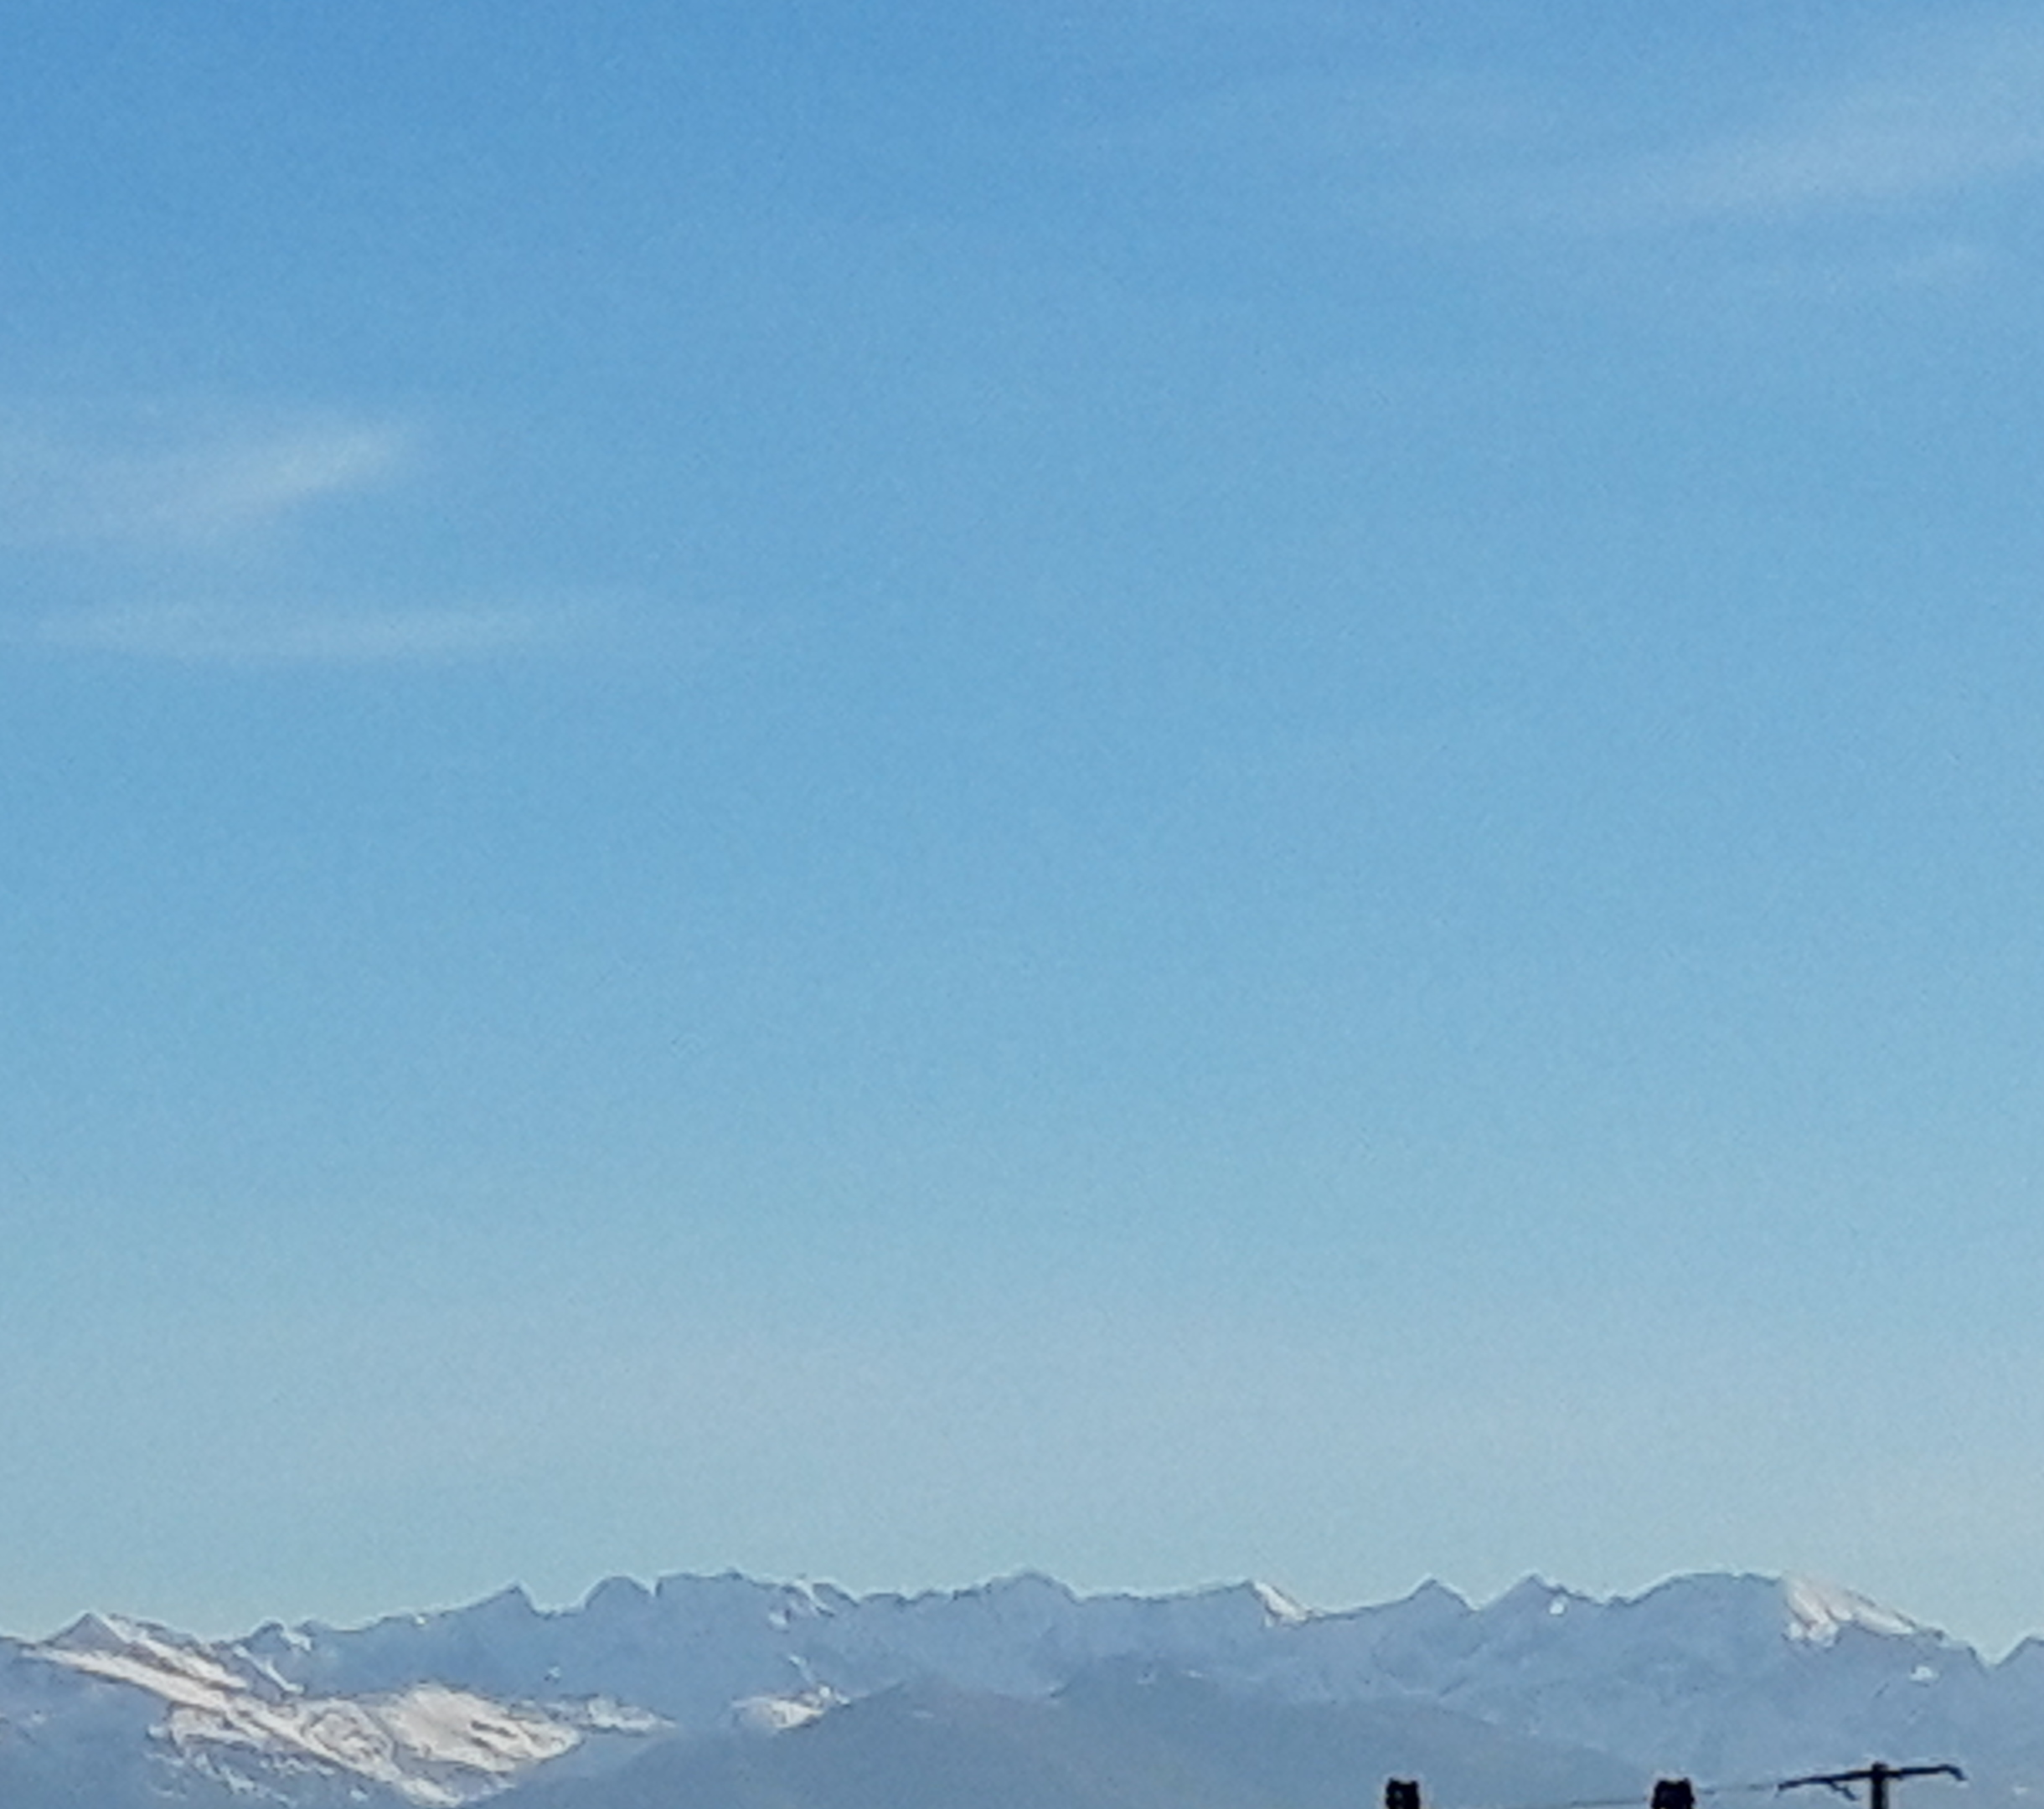
\includegraphics[width = 150pt]{Images/Montagne.jpg}
     \caption{Image T}
      \end{minipage}\hfill
   \begin{minipage}{0.48\textwidth}
     \centering
     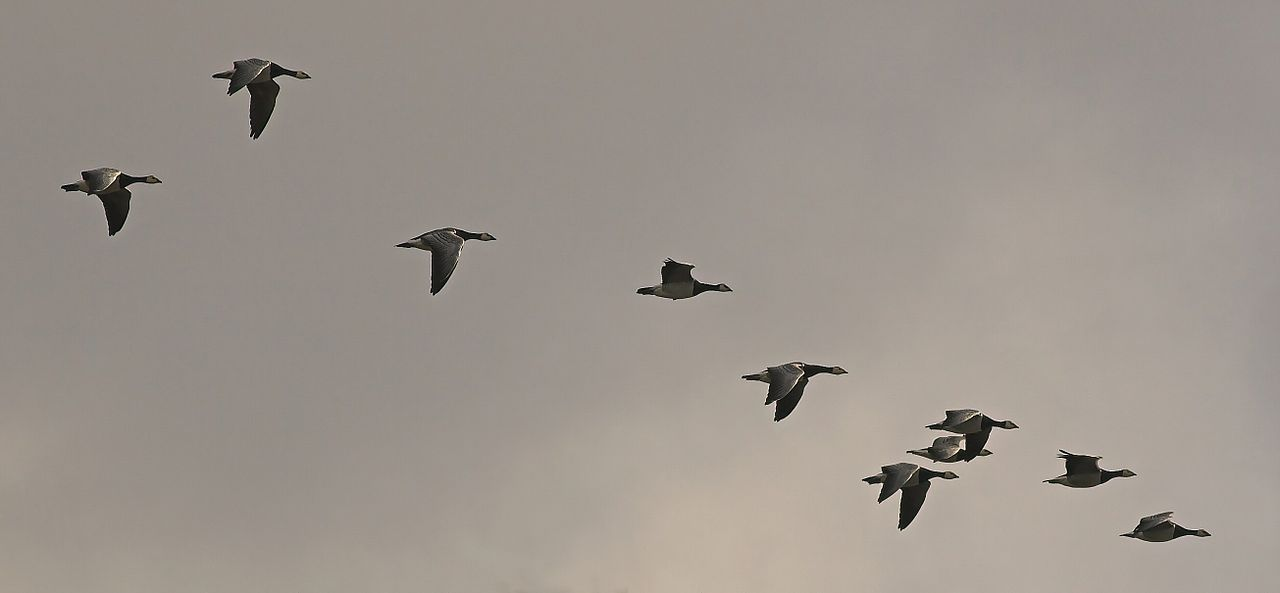
\includegraphics[width= 150pt]{Images/Oiseau.jpg}
     \caption{Image S}\label{Fig:Data2}
   \end{minipage}
\end{figure}

L'objectif est d'incruster toute ou partie de l'image S dans l'image T. En terme de manipulations, cela consiste à effectuer un copier/coller ou encore un clônage de la seconde image dans la première.
Le résultat que nous attendons pour une incrustation "réussie" est un résultat comme celui présenté ci-dessous : 
    
\begin{center}
\begin{figure}[!htb]
   \centering
     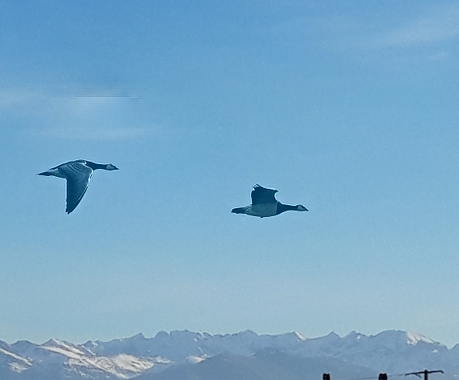
\includegraphics[width = 150pt]{Images/clonage_done.png}
     \caption{Image  finale attendue}
\end{figure}
\end{center}
Cette image est extraite d'une simulation effectuée sur \url{'demo.ipol.im/demo/163/'}. Nous comparerons les images obtenues à l'aide nos algorithmes avec celle-ci à la fin de ce rapport.\newline
\paragraph{Remarques}
Ce résultat est réussi parce qu'il semble naturel, les frontières entre l'image collée et l'arrière plan sont très peu visibles et ont été estompées, les oiseaux présents dans la première image n'ont pas été déformés et semblent faire parti de l'image. 
Mais comment obtenir un tel résultat ?
\newline
Reprenons nos deux images séparées, T et S et commençons par effectuer un simple copier/coller. Certains pixels de T sont donc écrasés par ceux de S. En effectuant cette manipulation voici l'image que nous devrions obtenir : 
\begin{center}
\begin{figure}[H]
     \centering
     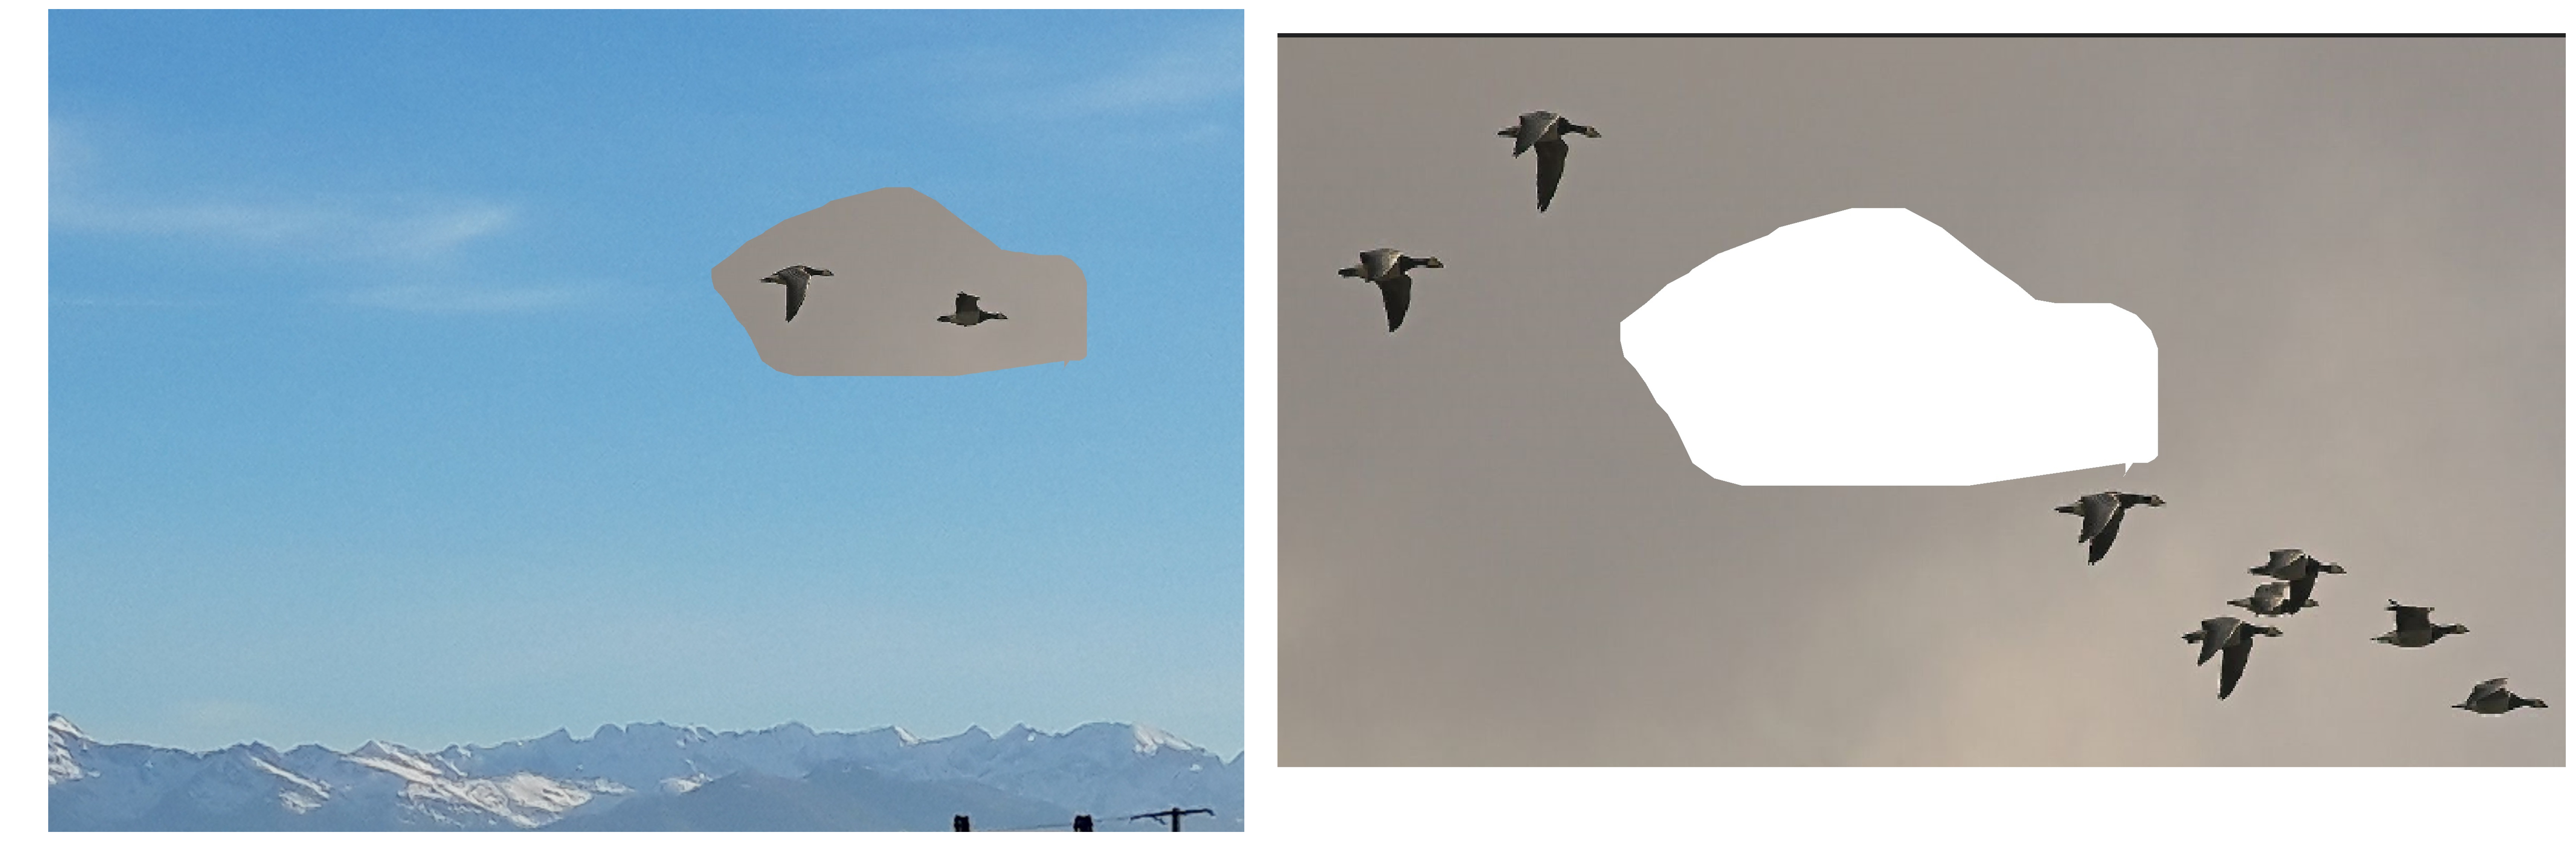
\includegraphics[width = 200pt]{Images/collage1.jpg}
     \caption{Simple copier/coller}
\end{figure}
\end{center}

Ce résultat n'est bien entendu pas convenable et bien loin de l'image finale attendue. Le découpage et le collage entre l'arrière-plan et l'image "objet" sont beaucoup trop visibles, les couleurs ne sont pas les mêmes et incohérentes. Nous souhaitons obtenir un résultat beaucoup plus naturel, comme écrit plus haut. Cette simple manipulation n'est donc pas suffisante pour effectuer le clônage cohérent  d'une image dans une autre. \newline

Il semble évident de vouloir modifier l'image finale obtenue ci-dessus afin qu'elle paraisse la plus naturelle possible.
Nous verrons tout au long de ce rapport, quels sont les changements à effectuer, et comment la résolution d'une équation aux dérivées partielles,l'équation de Poisson, nous permet d'obtenir un bien meilleur résultat. Nous implémenterons trois algorithmes permettant de résoudre le problème posé, et comparerons les résultats obtenus à l'aide de ceux-ci
%%%%%%%%%%%%%%%%%%%%%%%%%%%%%%%%%%%%%%%%%%%%%%%%%%%%%%%%%%
%           TRADUCTION SOUS FORMES MATHEMATIQUES         %
%%%%%%%%%%%%%%%%%%%%%%%%%%%%%%%%%%%%%%%%%%%%%%%%%%%%%%%%%%

\subsection{Problème mathématique associé}

Comme écrit plus haut nous souhaitons apporter des modifications au précédent collage afin qu'il corresponde au mieux à nos attentes. En réalité nous ne souhaitons pas modifier l'entièreté de l'image mais seulement un "sous-domaine" correspondant à l'endroit du collage. Pour ce faire, considérons I, la partie de l'image finale à modifier. Nous pouvons ainsi représenter le problème sous forme schématique. 
\begin{center}
    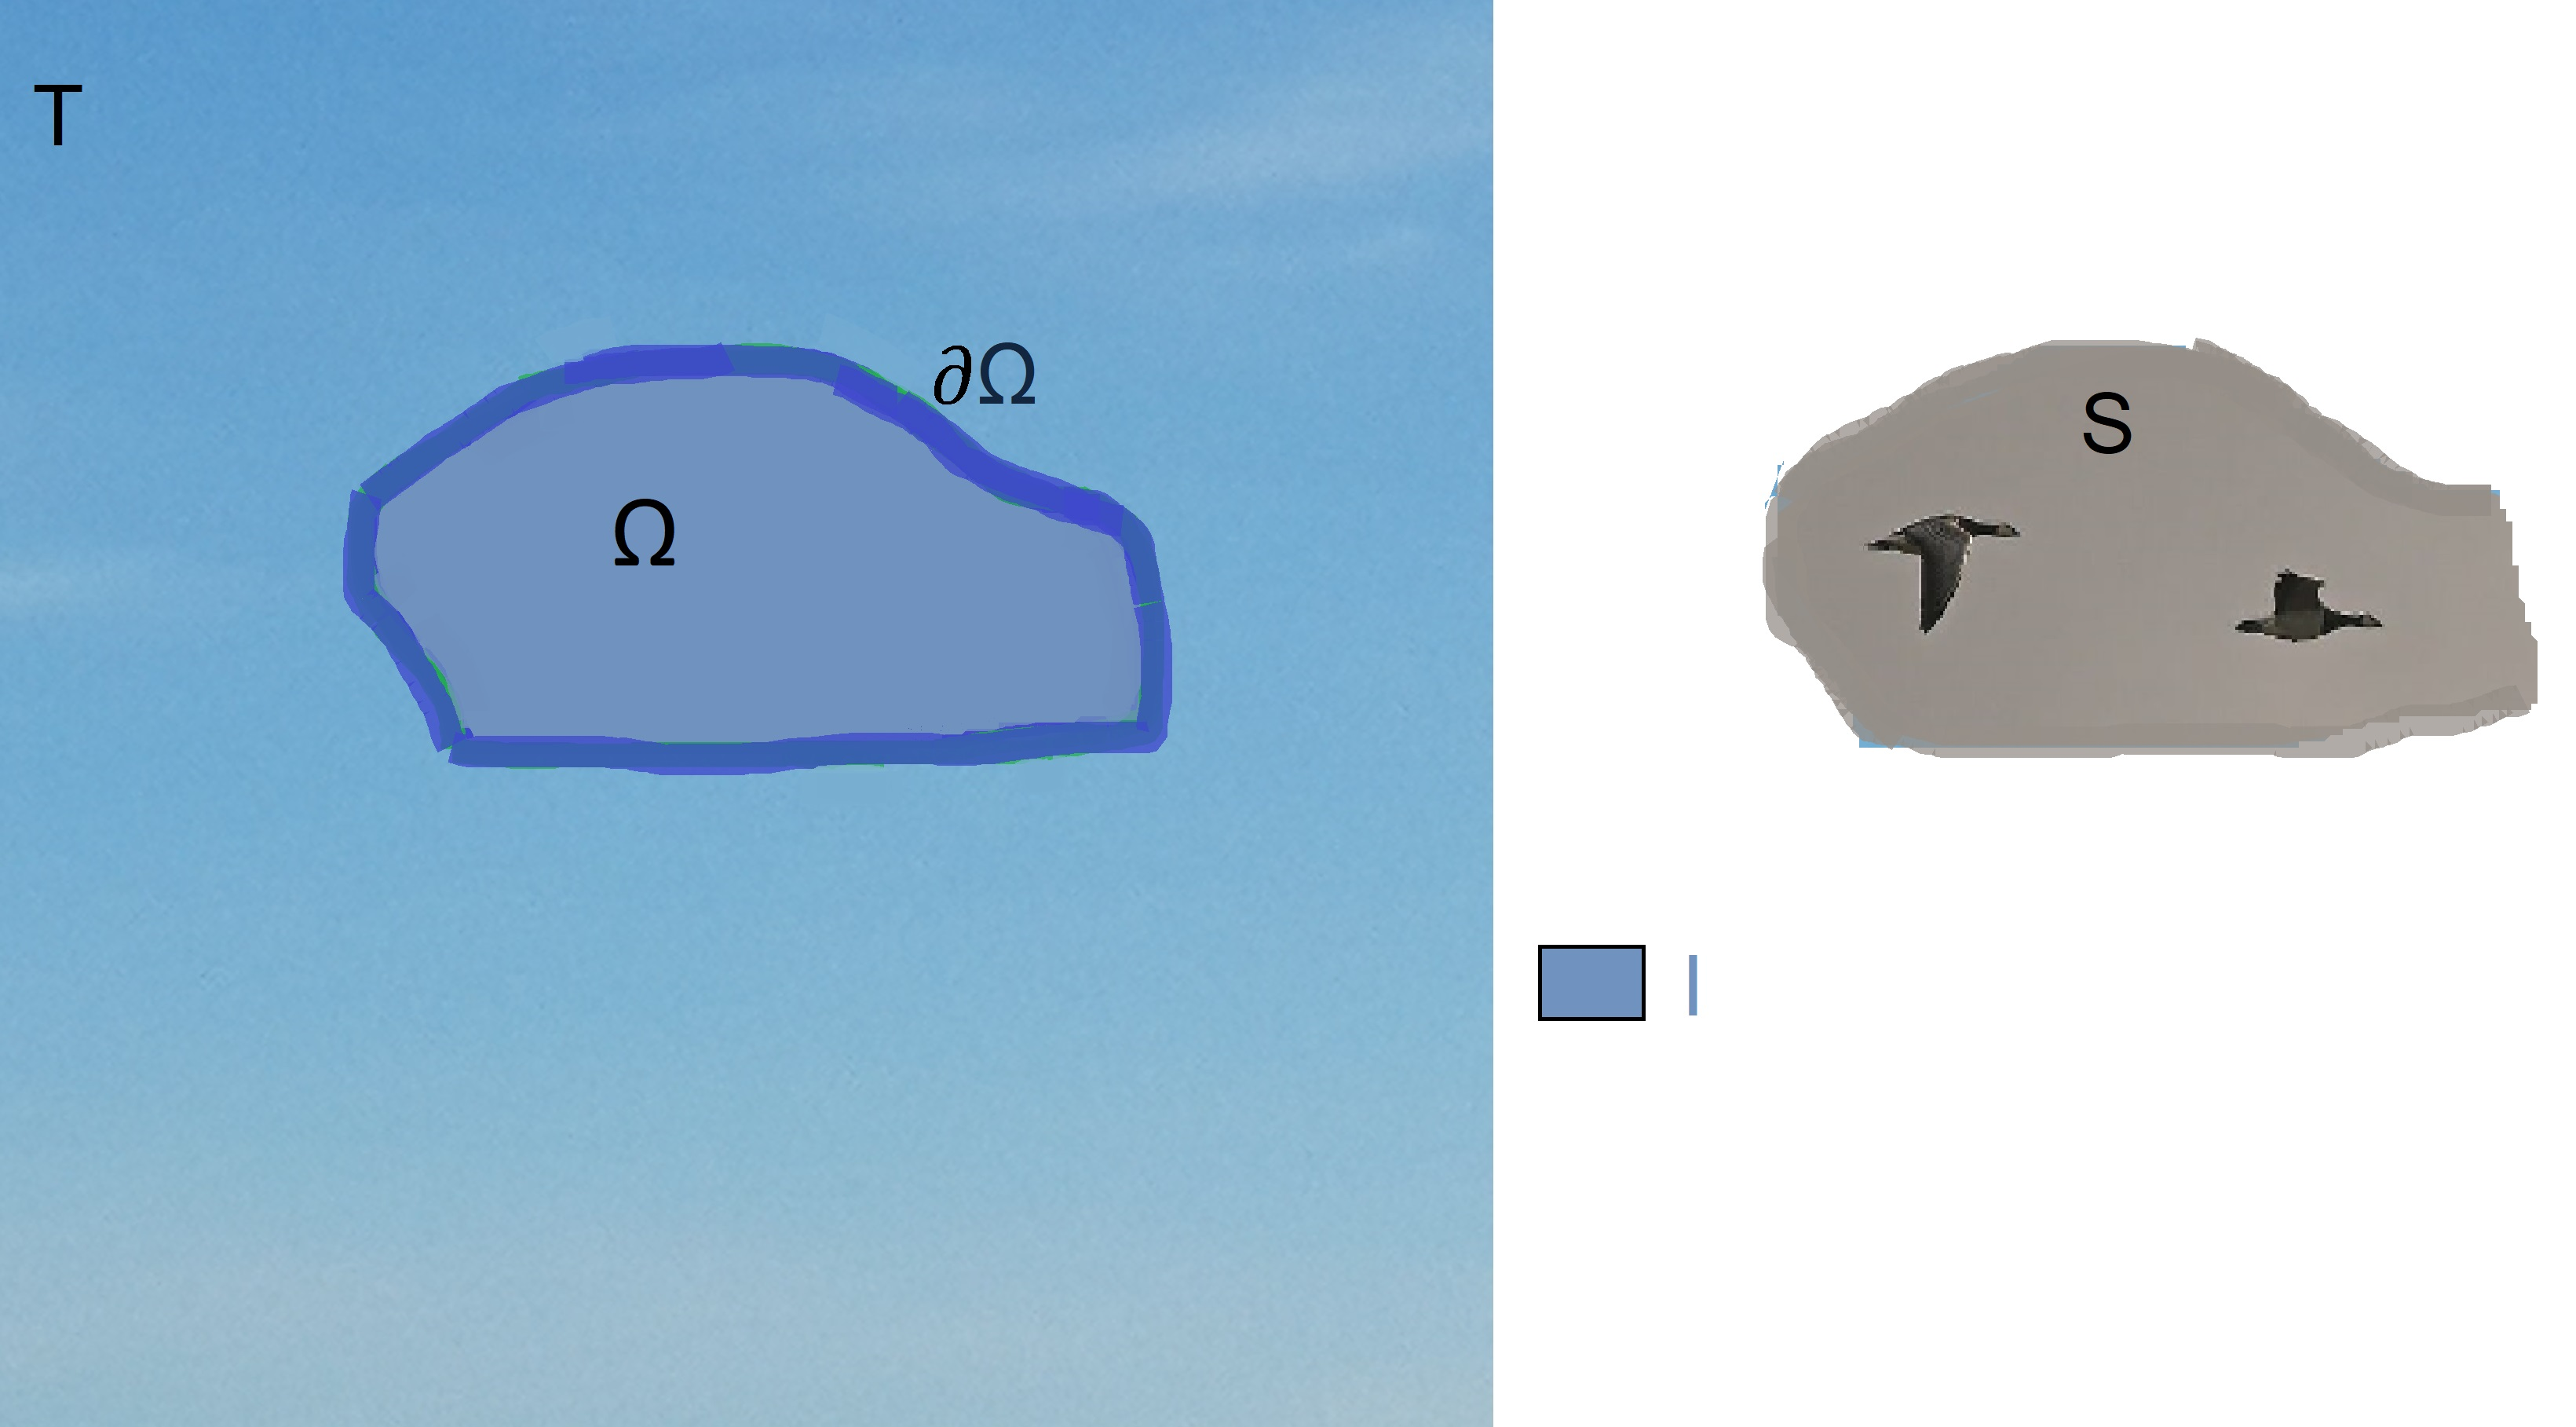
\includegraphics[width = 200pt]{Images/Schee.jpg}
\end{center}

Ici : 
\begin{itemize}
    \item T est l'image "Target", l'image destination, l'image sur laquelle s'effectuera le collage, l'arrière plan. 
    \item S est l'image "Source", l'image que nous souhaitons coller.
    \item $\Omega$ est le domaine dans lequel se trouvent nos inconnues.
    \item $\partial \Omega$ est la frontière de $\Omega$.
    \item I est notre inconnue, la partie de l'image que nous ne connaissons pas et que nous voulons remplir.
\end{itemize}

Nous souhaitons donc trouver une fonction I qui satisfasse un certain nombre de critères, afin de correspondre au résultat attendu.  
Cette fonction représente la partie modifiée de notre image. Mais quelles sont les conditions qu'elle doit remplir pour que le rendu soit le meilleur possible? Notre nouvelle image I doit-elle être plus proche de l'image collée S, ou de l'image d'arrière-plan T ? \newline
Pour répondre à cette question, reprenons le problème de départ. \newline

Pour que l'image obtenue s'incruste parfaitement,il faut que celle-ci dénature le moins possible les deux images sélectionnées au départ. En effet, nous devons garder les détails de l'image que nous voulons coller, S, ne pas modifier les variations qu'elle pourrait posséder comme par exemple, les contours ou les objets, lui appartenant.Nous devons donc pouvoir retrouver les informations présentes dans celle-ci. Par conséquent, il faut que les objets ou contours présents dans $I$ soient presque identiques à ceux de S.\\
Rappelons qu'en traitement d'image, les variations d'une image peuvent être obtenues en calculant le gradient de celle-ci. En effet, une variation peut-être représentée comme un changement "brutal" d'intensité entre deux pixels. Le gradient d'une image étant numériquement obtenu en effectuant la différence entre des pixels voisins : si celle-ci est élevée alors il y a une fort changement d'intensité entre eux, (par exemple un pixel noir et un autre blanc), et donc possiblement la présence d'un contour. Par conséquent, un fort changement d'intensité, implique un fort gradient. Au contraire, l'absence de variations entraîne un gradient presque nul. Son calcul permet entre autre de détecter les contours d'une image.\\
Nous souhaitons ici, que les contours de l'image finale soient très proches de l'image à coller. Mathématiquement, nous voulons donc une fonction I dont le gradient est le plus proche possible, ou identique à celui de l'image collée, S. Nous cherchons donc :
\begin{center}
    $$ min \iint_\Omega || \nabla I_{x,y} - \nabla S_{x,y}||^2 dxdy$$
\end{center} 

Mais les "frontières" entre l'image collée et l'image d'arrière-plan T, ne doivent pas non plus être visibles, il faut donc que les pixels se situant sur cette partie là, i.e $\partial \Omega$, soient le plus proches possible de T .  Nous voulons donc, mathématiquement, chercher la fonction I qui vérifie: 
\begin{center}
    $I_{(x,y)} = T_{x,y} \ sur\ \partial \Omega$
\end{center}

Répondre au problème implique donc de résoudre un problème variationnel classique auquel des conditions sur le bord de Dirichlet sont ajoutées. 
Réécrivons le problème mathématique que nous cherchons à résoudre :  

\begin{center}
\begin{equation}
\left\{
\begin{aligned}
 min \iint_\Omega || \nabla I_{x,y} - \nabla S_{x,y}||^2 dxdy\\
 I_{(x,y)} = T_{x,y} \ sur\ \partial \Omega
\end{aligned}
\right.
\end{equation}
\end{center}


\subsection{Résolution et équivalence avec l'équation de poisson}
Pour résoudre cette équation, nous devons trouver le minimum de la fonction g suivante  : 
\begin{center}
\begin{equation}
\begin{aligned}
g(I) = \int_\Omega || \nabla I(x) - v(x)||^2 dx\\
\end{aligned}
\end{equation}
\end{center}
Si g admet un minimum alors, celui-ci annule son gradient. 
\subparagraph{Calcul de $\nabla g(I)$ }
À l'aide des formules de Taylor-Young à l'ordre 1 :\\
Soit f une fonction: $\mathbb{R}^n\rightarrow \mathbb{R}$ et $u \in \mathbb{R}^n$, tel que $||u||=1$ :
\begin{equation*}
\begin{aligned}
f(x_0+\epsilon u) = f(x_0) +\epsilon \left<\nabla f(x_0), u\right> + o(\epsilon)\\
\end{aligned}
\end{equation*}
En appliquant ces formules à notre cas :
\begin{equation*} 
\begin{aligned}
    g(I+\epsilon u) -g(I) =  \int_\Omega || \nabla (I+\epsilon u) - v||^2 - ||\nabla I -v ||^2 dx\\
\end{aligned}
\end{equation*}
En  développant : 
\begin{equation*} 
\left.
\begin{aligned}
    g(I+\epsilon u) -g(I) &=  \int_\Omega || \nabla I - v||^2+ ||\nabla \epsilon u||^2 +2(\nabla I - v)\times \epsilon \nabla u  - ||\nabla I -v ||^2 dx\\
  &=  \int_\Omega \epsilon ^2||\nabla u||^2 +2(\nabla I - v)\times \epsilon \nabla u dx\\
    & = 2\int_\Omega (\nabla I - v) \times (\nabla \epsilon u ) + O (\epsilon^2) \\ 
    & = 2\left<\nabla I - v, \nabla \epsilon u \right> + O (\epsilon^2) \\ 
      &  =   2\epsilon<\nabla I - v,  \nabla u> + O (\epsilon^2) \\ 
         &  = 2\left<\nabla I - v,  \nabla u \right> + O (\epsilon)\\ 
    & =  -2 <div(\nabla I - v), u > + O (\epsilon)\\
\end{aligned}
\right.
\end{equation*}
Par identification, le gradient de g vaut 
\begin{center}
		$\nabla g(I) = -2(\Delta I-div( v))$
\end{center} 
Le minimum de g annule son gradient donc on cherche I tel que : 
\begin{center}
		$0= (-\Delta I+div( v))$
\end{center}
Ici v = $\nabla S$ 
\begin{center}
		$\Delta I =div(\nabla S)$\\
		$\Delta I = \Delta S$
		
\end{center} 

Trouver le minimum de (2) revient donc à résoudre l'équation : 
\begin{center}
$\Delta I = \Delta S$
\end{center}
En remplaçant dans (1). On obtient le problème suivant : 
\begin{center}
    \begin{equation*}
        \left\{
        \begin{aligned}
         \Delta I = \Delta S  \ sur \  \Omega \\
          I = T \ sur \  \partial \Omega
        \end{aligned}
        \right.
    \end{equation*}
\end{center}
qui n'est autre que l'équation de Poisson, avec conditions aux bords de Dirichlet. 
Ainsi : résoudre le problème variationnel est équivalent à résoudre l'équation de poisson avec conditions aux bords de Dirichlet. Nous décrirons dans ce rapport 3 manières de résoudre cette équation. 


\section{Résolution}
Nous verrons dans un premier temps, comment résoudre cette équation à l'aide de discrétisation et de différences finies. Puis nous résoudrons celle-ci à l'aide des transformées de Fourier. 
Rappelons que nous souhaitons résoudre l'équation de Poisson suivante : 
\begin{center}

\begin{equation*}
    \left \{
    \begin{aligned}
    \Delta I = \Delta S \ sur \ \Omega\\
    I = T \ sur \ \partial \Omega
    \end{aligned}
    \right.
\end{equation*}
\end{center}
%Nous cherchons ici à déterminer $\Delta I$ que nous ne connaissons pas. Au contraire, $\Delta S $ est facile à calculer, car nous connaissons S, et les valeurs de ses pixels. 
%\newline
%Rappelons que le Laplacien d'une fonction I(x,y) s'écrit de cette façon : 
%\begin{center}
%\begin{equation*}
%    \Delta I(x,y)  = \frac{\partial^2 I}{\partial x^2}+ \frac{\partial ^2 I}{\partial y^2}
%\end{equation*}
%\end{center}

\subsection{Discrétisation \cite{Image}}
Avant de discrétiser les Laplaciens de nos deux images, il faut définir le maillage que nous allons utiliser.
 
\subsubsection{Qu'est qu'une image}
Une image peut être représentée comme une succession de pixels. En traitement d'image, ce sont d'ailleurs sur ces pixels que le traitement est effectué. Leur modification entraîne la modification de l'image globale.Nous verrons donc une image comme la succession de pixels et nous pouvons la représenter comme une grille, dans laquelle chaque carré représente un pixel.  Schématiquement, nous pourrions donc découper notre image comme ci-dessous
    \begin{figure}[!htb]
        \centering
       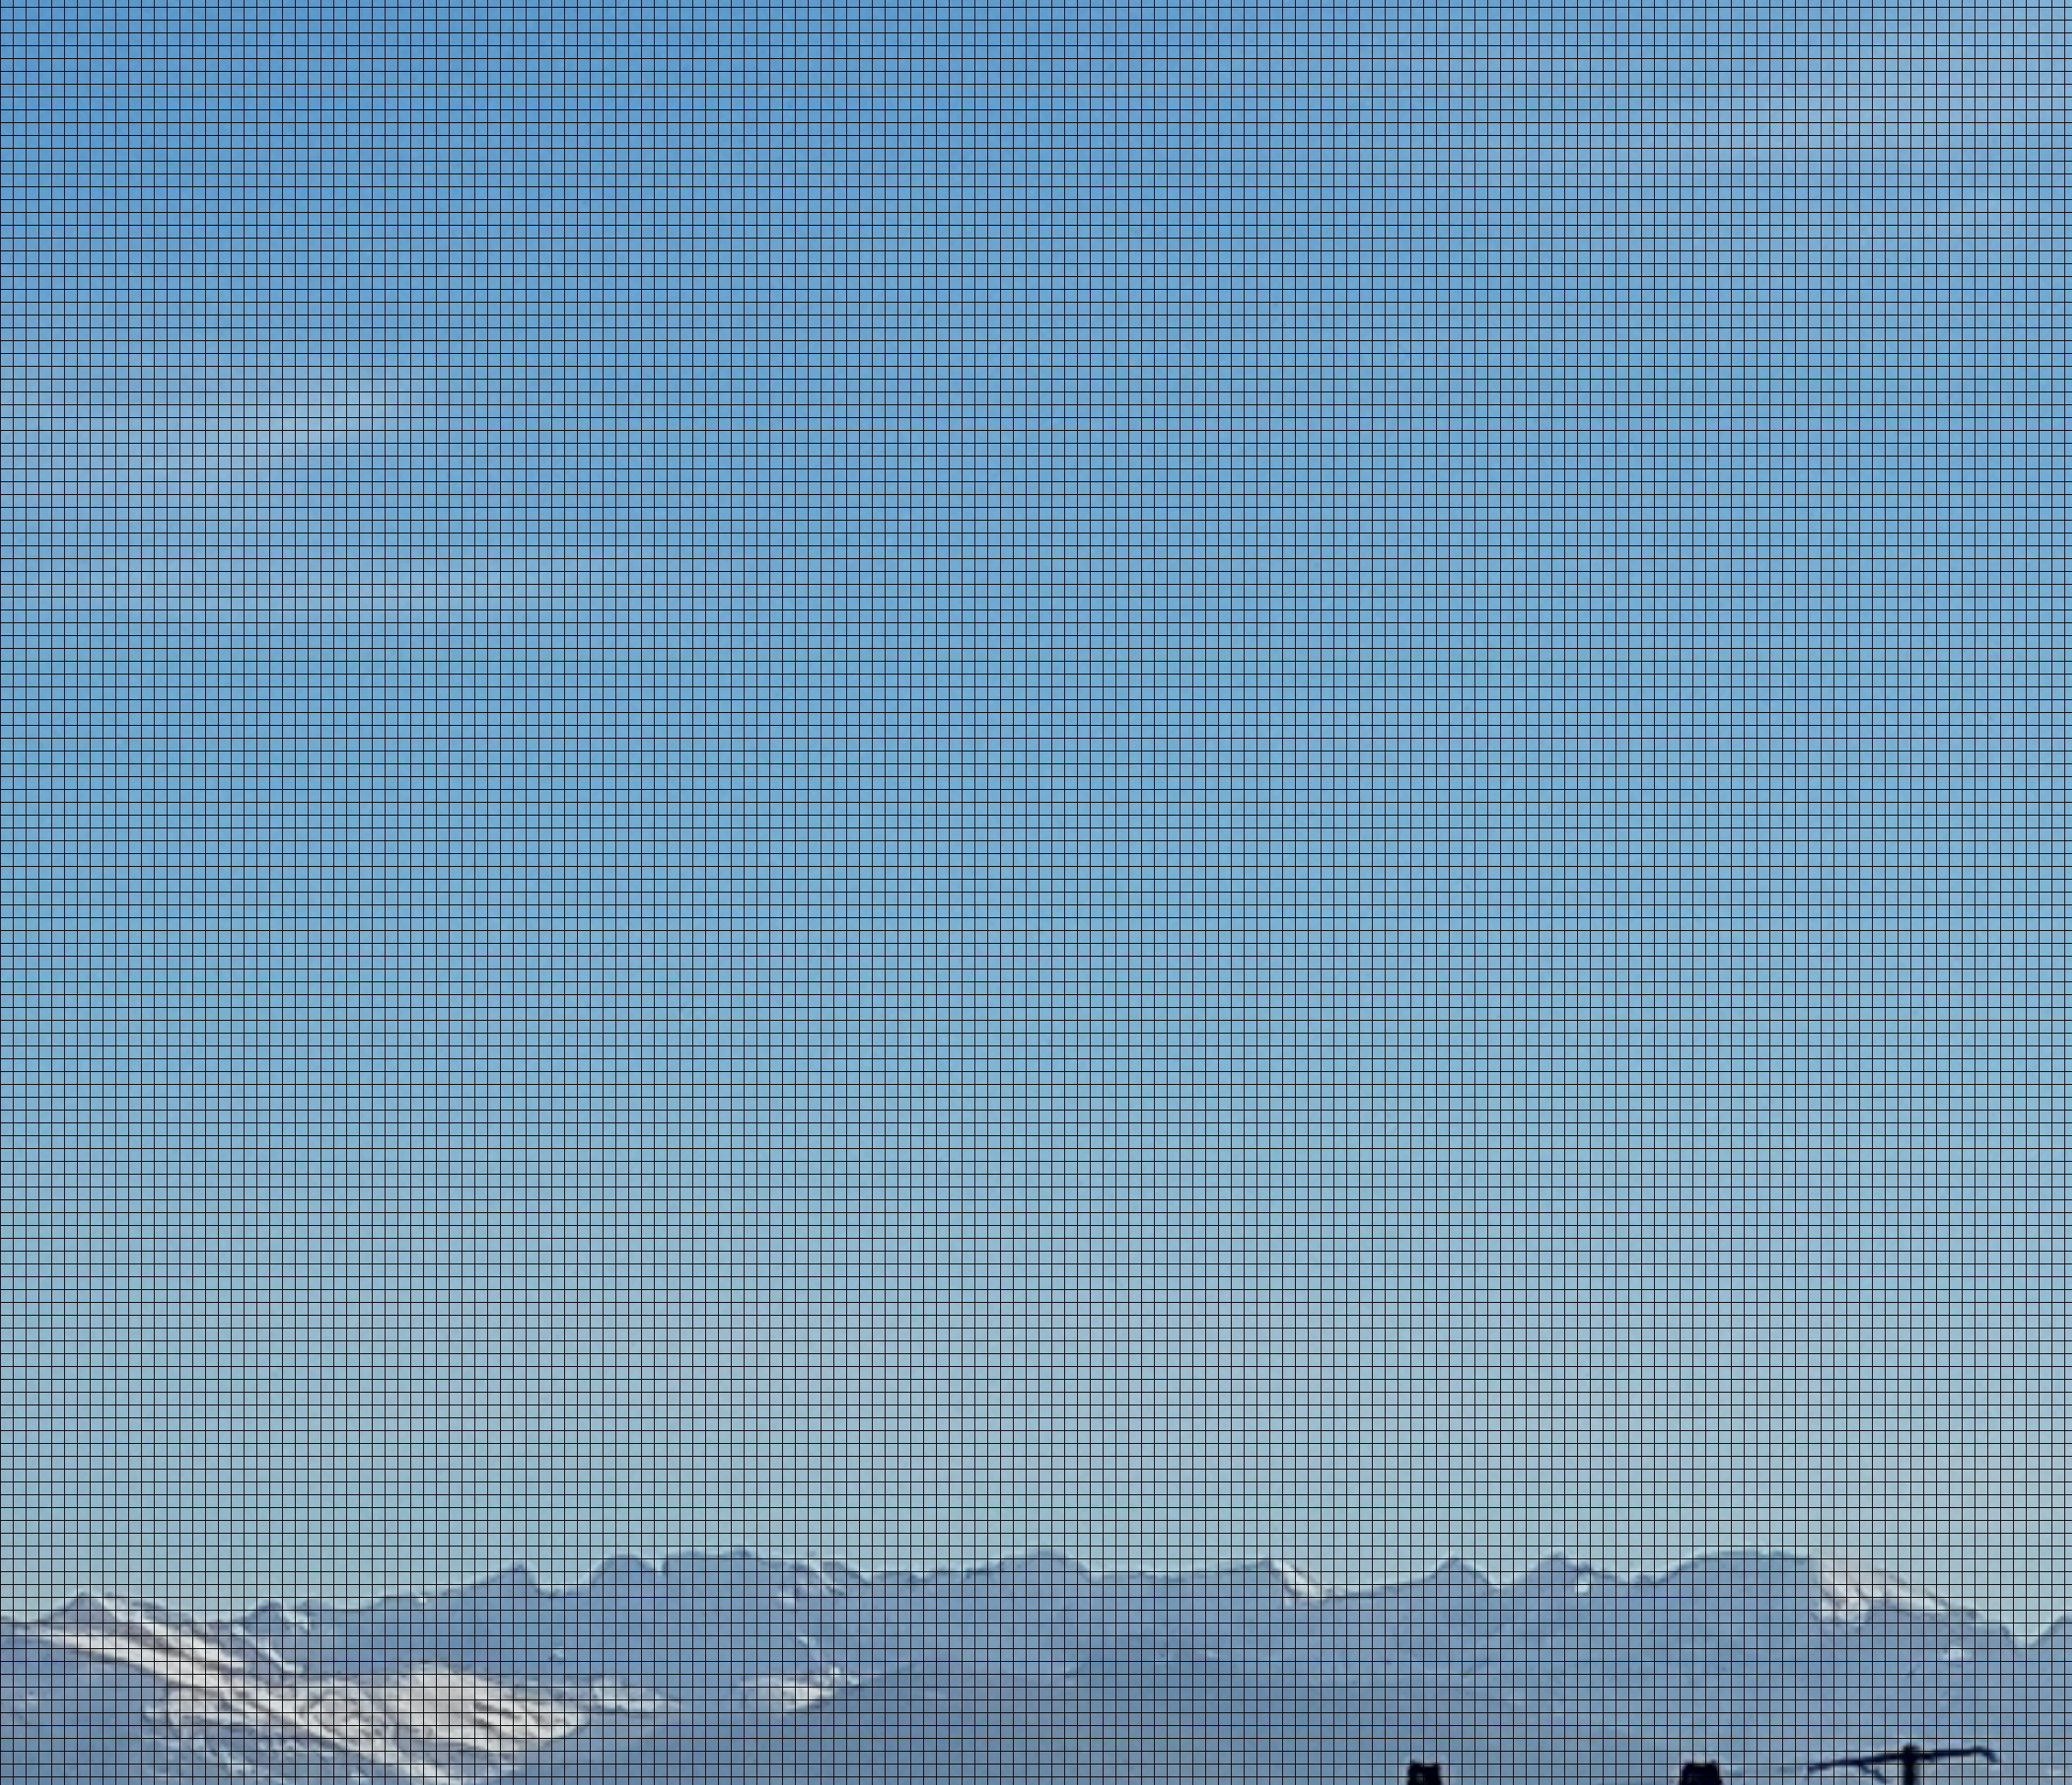
\includegraphics[scale = 0.07]{Images/Montagne_grille.jpg}
        \caption{Maillage d'une image}
        \label{fig:my_label}
    \end{figure}
Nous numéroterons les pixels suivant la règle suivante. Le premier pixel est situé en haut en gauche, puis il suffit de parcourir la grille comme ci-dessous : 

	\begin{figure}[!htb]
	\centering
	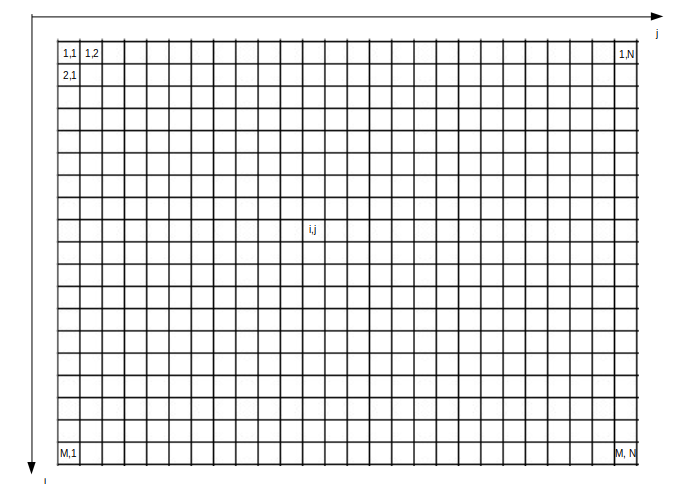
\includegraphics[scale=0.5]{Images/grille.png}
	\caption{Parcours d'une grille}
	\label{fig:my_label}
	\end{figure}
Les pas d'espaces sont donc égaux et valent 1. Dans la suite nous considérons que notre image est de taille $N \times M$.
\newpage


\subsection{Les différents opérateurs nécessaires}
Nous utiliserons certains opérateurs que nous définissons ici afin de ne pas alourdir les différentes sections. 
\subparagraph{Le gradient}

\subparagraph{Le Laplacien}
Le Laplacien peut s'écrire de la forme : 

\begin{center}
\begin{equation*}
    \Delta I(x,y)  = \frac{\partial^2 I}{\partial x^2}+ \frac{\partial ^2 I}{\partial y^2}
\end{equation*}
\end{center}

\subsection{Méthode des différences finies}
Nous cherchons à résoudre  : 
\begin{center}

\begin{equation*}
    \left \{
    \begin{aligned}
    \Delta I = \Delta S \ sur \ \Omega\\
    I = T \ sur \ \partial \Omega
    \end{aligned}
    \right.
\end{equation*}
\end{center}

En utilisant la méthode des différences finie, commençons par discrétiser le Laplacien.
Pour discrétiser celui-ci, il faut donc commencer par discrétiser $\frac{\partial^2 I}{\partial x^2}$ et  $\frac{\partial^2 I}{\partial y^2}$. 

\subparagraph{Discrétisation des dérivées secondes :}

A l'aide des formules de Taylor à l'ordre 2 ci-dessous : 
\begin{equation*}
\begin{aligned}
    I(x+h,y) = I(x,y)+h\times \frac{\partial I(x,y)}{\partial x}+ \frac{h^2}{2} \times \frac{\partial ^2 I(x,y)}{\partial x^2} + o(h^3) \\
    I(x-h,y) =I(x,y)- h\times  \frac{\partial I(x,y)}{\partial x}+ \frac{h^2}{2} \times \frac{\partial^2 I(x,y)}{\partial x^2} + o(h^3)
\end{aligned}
\end{equation*}


Et en effectuant la somme de ces deux équations, nous obtenons une discrétisation possible de $\frac{\partial ^2 I(x,y)}{\partial x^2}$:  
\begin{equation*}
    \frac{\partial ^2 I(x,y)}{\partial x^2} =\frac{1}{h^2}\left( I(x+h,y) + I(x-h,y) - 2\times I(x,y)\right)
\end{equation*}

\subsubsection{Discrétisation du Laplacien}
Comme le Laplacien n'est autre que la somme de $\frac{\partial ^2 I(x,y)}{\partial x^2}$ et$\frac{\partial ^2 I(x,y)}{\partial y^2}$, une discrétisation possible de celui-ci s'écrit de la forme  : 
\begin{equation*}
    \Delta I(x,y) =  \frac{I(x+h,y) + I(x-h,y) - 2\times I(x,y)}{h^2}  + \frac{I(x,y+k) + I(x,y-k) - 2\times I(x,y)}{k^2} \\
\end{equation*}

Les pas d'espaces h et k étant égaux à 1, nous pouvons écrire une discrétisation du Laplacien  :
\begin{equation*}
     \Delta I(x,y) =  I(x+1,y) + I(x-1,y)+ I(x,y+1) + I(x,y-1) - 4\times I(x,y)  \\
\end{equation*}

\subparagraph{Application à une image }
Afin de calculer le Laplacien du pixel I(i,j),il est donc nécessaire d'avoir la connaissance de ses pixels voisins que nous nommerons par la suite U(p), D(own), L(eft), R(ight) pour les pixels I(i-1,j), I(i+1,j), I(i,j-1), I(i,j+1). 

\begin{center}
    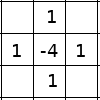
\includegraphics[scale = 0.8]{Images/Laplacian.png}
\end{center}

\subsubsection{Résolution de l'équation de Poisson} 
Soit $g(x,y) = S(x+1,y) + S(x-1,y)+ S(x,y+1) + S(x,y-1) - 			4\times S(x,y)$\\
Résoudre $\Delta I(x,y) = \Delta S(x,y)$ sur $\Omega$ est équivalent à résoudre :\\
\begin{center}
\begin{equation*}
    \left \{
    \begin{aligned}
    I(i+1,j) + I(i-1,j)+ I(i,j+1) + I(i, j-1) - 4\times 			I(i,j)= g(i,j)\\ pour (i,j)\in \Omega \\
    I(i,j) = T(i,j) \ pour \ (i,j) \in \partial \Omega
    \end{aligned}
    \right.
\end{equation*}
\end{center}
Nous devons donc résoudre un système à $M\times N $ inconnues.
\begin{equation}
\left\{
\begin{aligned}
I(1,1) = T(1,1)\\
I(3,2)+I(1,2)+ I(2,3)+I(2,1)-4I(2,2) =g(2,2) \\
I(3,3)+I(1,3)+ I(2,4)+I(2,2)-4I(2,3) =g(2,3)             \\
... \\
I(M,N-1)+I(M-2,N-1)+ I(M-1,N)+I(M-1,N-2) =g(M-1,N-1)\\
I(M, N) = T(M, N)
\end{aligned}
\right.
\end{equation}

Afin de résoudre ce système, il est plus facile de l'écrire sous forme matricielle. Nous devons donc résoudre un système de la forme AI = b et sa solution est  :  $I = A^{-1}\times b$.
Avec : 
\begin{itemize}
\item A une matrice carrée de taille ($M\times N$, $M\times N$)
\item I un vecteur colonne de taille ($M\times N$,1)
\item b un vecteur colonne de taille ($M\times N$,1)
\end{itemize}
Voici donc à quoi ressemble le système que nous souhaitons résoudre :
\begin{center}

\begin{equation}
\left.
\begin{aligned}
\begin{pmatrix}
	-4 & 1 & 0 & ...& 0 & 1 & 0...&0& ... & 0\\
	1 & -4 & 1 & 0 & ... & 0 &1 &0&....&0\\
	0 & 1 & -4 & 1 & 0&... &0 &1 &0&...\\
	&...\\
	1 & 0 &... &1 &-4 &1 &0...& 0& 1 & 0\\
\end{pmatrix}
\begin{pmatrix}
I(1,1)\\
I(2,1)\\
...\\
I(1,2)\\
I(2,2)\\
....\\
I(M, N)
\end{pmatrix}
= 
\begin{pmatrix}
g(1,1)\\
g(2,1)\\
...\\
g(1,2)\\
g(2,2)\\
....\\
g(M, N)
\end{pmatrix}
\end{aligned}
\right.
\end{equation}
\end{center}

\subparagraph{Transformation de l'image}
Afin de pouvoir résoudre ce système, I doit être un vecteur colonne. Or dans notre cas, I est une matrice de taille (M,N). Le nouveau vecteur I, est la concaténation des colonnes de l'image I, comme ci dessous.

\subparagraph{Ecriture de la matrice du système}
Pour remplir la matrice A dont nous avons besoin.Premièrement

\subparagraph{Ecriture de vecteur}
Après avoir calculé le Laplacien de l'image S, le vecteur b est obtenu en concaténant les colonnes de l'image $\Delta S$. 

\subparagraph{Exemple simple}
Considérons l'image S ci-contre que nous souhaitons coller. 
\begin{figure}[!h]
\centering

\includegraphics[scale=0.1]{Images/square.png}
\caption{Image à coller}
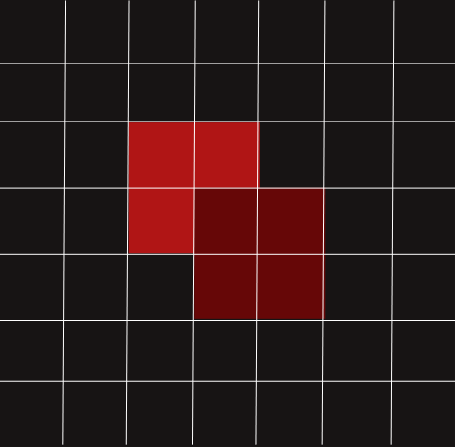
\includegraphics[scale=0.1]{Images/pix.png}
\caption{Vue grille pixel}
\end{figure}
Nous souhaitons ici coller les deux carrés rouge sur une image que nous nommerons T. Commençons par sélectionner la zone que nous souhaitons coller, comme ci-dessous. 
\begin{figure}[!h]
\centering
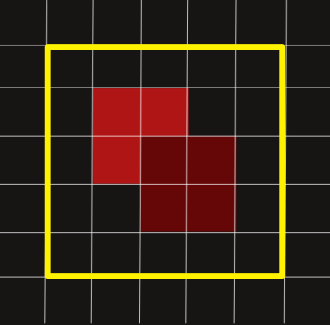
\includegraphics[scale=0.3]{Images/carre_selection.png}
\caption{Sélection à coller}
\end{figure}

\begin{figure}[!h]
\centering
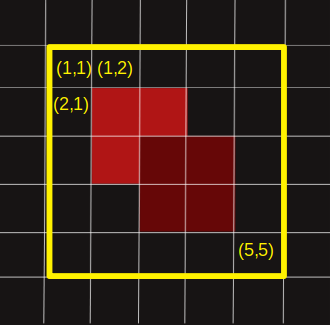
\includegraphics[scale=0.3]{Images/numerote.png}
\caption{Numérotation des pixels}
\end{figure}


\paragraph{Construction du système}
Ici les pixels avec la pastille verte sont sur $\delta \Omega$. On veut donc résoudre le système suivant :  
\begin{center}
\begin{equation}
\left\{
\begin{aligned}
I_{1,1} = T_{1,1}\\
...\\
I_{5,1} = T_{5,1}\\
I_{1,2} = T_{1,2}\\
\Delta I_{2,2} = \Delta S_{2,2}\\
\Delta I_{3,2} = \Delta S_{3,2}\\
\Delta I_{4,2} = \Delta S_{4,2}\\
...\\
\end{aligned}
\right.
\end{equation}
\end{center}
Avec $\Delta I(i,j) = U+D+L+R-4I(i,j)$.\\
En écrivant ce système sous forme matricielle la matrice A est la matrice $25\times 25$ ci-dessous :  

\begin{figure}[!h]
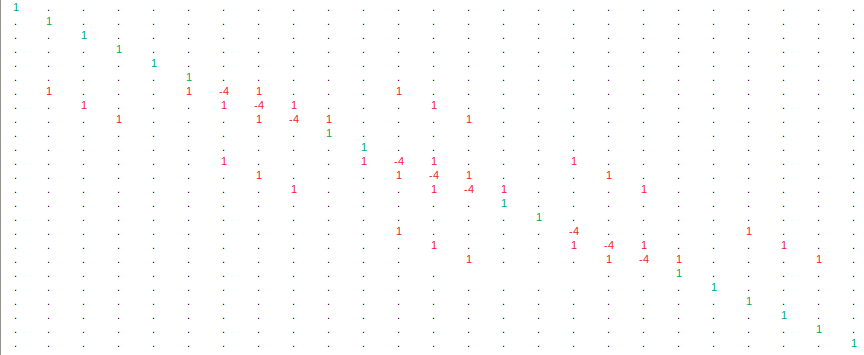
\includegraphics[scale=0.5]{Images/matrice.png}
\caption{Matrice du système}
\end{figure}

Le vecteur I est obtenu en concaténant les colonnes de la sélection, il est de taille($25\times 1$) : 
\begin{equation}
\begin{pmatrix}
I(1,1)\\
I(2,1)\\
...\\
I(5,1)\\
...\\
I(1,3)\\
...\\
I(5,3)\\
...\\
I(5,5)\\
\end{pmatrix}
\end{equation}
Enfin le vecteur b 

\begin{equation}
\begin{pmatrix}
T(1,1)\\
...\\
\Delta S(2,2)\\
...\\
T(5,2)\\
\Delta S(1,3)
...\\
T(5,3)\\
\Delta S(2,4)\\
...\\
\Delta S(4,4)\\
T(5,4)\\
...\\
\end{pmatrix}
\end{equation}
La solution I, s'écrit sous la forme $I = A^{-1}b$.


\subsection{Fourier \cite{Image}}
Avec cette seconde méthode nous allons résoudre l'équation de Poisson à l'aide de la transformée de Fourier. Avant de formuler la résolution de ce problème. Rappelons la définition des opérateurs dont nous aurons besoin dans la suite. \cite{Fourier}
\subsubsection{Rappel et définitions des opérateurs}
\paragraph{Transformée de Fourier (discrète)}
Soit F une fonction, sa transformée de Fourier peut s'écrire de la façon suivante : 
\begin{equation}
\begin{aligned}
\widehat{F}(x,y) = \sum_{k = 0}^{M-1} \sum_{l = 0}^{N-1} F(k,l) e^{-2\pi i\left(\frac{k\times x}{M}+\frac{l\times y}{N}\right)}
\end{aligned}
\end{equation}
Enfin, afin de retrouver la fonction initiale nous aurons besoin de la transformée de Fourier inverse : 
\begin{equation}
\begin{aligned}
F(k,l) = \frac{1}{MN} \sum_{x = 0}^{M-1} \sum_{y = 0}^{N-1} \hat{F}(x,y) e^{2\pi i \left(\frac{xk}{M}+\frac{yl}{N}\right)}
\end{aligned}
\end{equation}
\paragraph{Gradient}
Pour résoudre le problème nous avons besoin de calculer les Laplaciens des images. Nous nous placerons dans le domaine de Fourier, il est donc nécessaire de calculer la transformée de Fourier du Laplacien d'une fonction, et donc le gradient de celle-ci. 
F est toujours la fonction que nous souhaitons étudier. 
\begin{equation}
\begin{aligned}
\widehat{\nabla (F)}=
\begin{pmatrix}
\widehat{\frac{\partial F}{\partial k}}\\
\widehat{\frac{\partial F}{\partial l}}
\end{pmatrix}
\end{aligned}
\end{equation}
En dérivant l'expression ci-dessus par rapport à la première variable : 
\begin{equation}
\begin{aligned}
\frac{\partial F}{\partial k} &= \frac{1}{MN}\sum_{x = 0}^{M-1} \sum_{y = 0}^{N-1} \widehat{F}(x,y) e^{2\pi i\left(\frac{k\times x}{M}+\frac{l\times y}{N}\right)}\left(\frac{2\pi i x}{M}\right)\\
& = \left(\frac{2\pi i x}{M}\right)F(k,l)\\
\widehat{\frac{\partial F}{\partial k}} &= \left(\frac{2\pi i x}{M}\right)\widehat{F(k,l)}
\end{aligned}
\end{equation}
Le calcul est similaire pour $\widehat{\frac{\partial F}{\partial l}}$.\\
On a donc : 
\begin{equation}
\begin{aligned}
\widehat{\frac{\partial F}{\partial k}} = \left(\frac{2\pi i}{M}x\right) \widehat{F}\\
\widehat{\frac{\partial F}{\partial l}} = \left(\frac{2\pi i}{N}y\right) \widehat{F}\\
\end{aligned}
\end{equation}

\paragraph{Laplacien}
\begin{equation}
\begin{aligned}
\frac{\partial^2 F}{\partial k ^2} & = \frac{1}{MN} \sum_{x = 0}^{M-1} \sum_{y = 0}^{N-1} \widehat{F}(x,y) e^{2\pi i\left(\frac{k\times x}{M}+\frac{l\times y}{N}\right)}\left(\frac{2\pi i x}{M}\right)^2\\
& = \left(\frac{2\pi i x}{M}\right)^2 F(k,l)\\
\widehat{\frac{\partial^2 F}{\partial k^2}} &= \left(\frac{2\pi i x}{M}\right)^2\widehat{F(k,l)}
\end{aligned}
\end{equation}
On a donc : 
$\widehat{\Delta F} = \widehat{\frac{\partial^2 F}{\partial k^2}}+ \widehat{\frac{\partial^2 F}{\partial l^2}}$.
\begin{equation}
\widehat{\Delta F} = \left(\frac{2\pi i x}{M}\right)^2 \widehat{F}+\left(\frac{2\pi i y}{N}\right)^2 \widehat{F}
\end{equation}

\subsubsection{Résolution avec la méthode Fourier}
La résolution dans le domaine de Fourier nécessite quelques changements. Cette méthode ne fonctionnant que sur un domaine rectangulaire, nous devons donc modifier le domaine $\Omega$.\\
Rappelons que nous voulons résoudre le problème suivant :
\begin{equation}
\left\{
\begin{aligned}
\Delta I(x,y) = \Delta S(x,y) \ si \ (x,y) \in \Omega\\
I(x,y) = T(x,y) \ si \ (x,y) \notin \Omega
\end{aligned}
\right.
\end{equation}

Nous voulions que le laplacien de I à l'intérieur de $\Omega$ corresponde à celui de S. En considérant le nouveau domaine $\Omega_2$ comme étant l'image entière, il faudrait donc que le Laplacien de I soit très proche du laplacien de $T \cup S$. Mais dans ce cas, nous aurions un fort gradient sur $\partial \Omega$, (le  changement d'intensité entre T et S étant fort). Il faut donc reconsidérer le problème précédent. \\
La nouvelle hypothèse que nous pouvons faire est donc la suivante : $\nabla I$ doit être très proche de $\nabla S$ dans $\Omega$ mais aussi très proche de $\nabla T$ dans $\Omega_2 \backslash \Omega$. En notant V : 
\begin{equation}
V = 
\left\{
\begin{aligned}
\nabla S(x,y) \ si \ (x,y) \in \Omega\\
\nabla T(x,y) \ si \ (x,y) \notin \Omega
\end{aligned}
\right.
= \begin{pmatrix}
V_1\\
V_2
\end{pmatrix}
\end{equation}
\begin{figure}[!htb]
   \begin{minipage}{0.5\textwidth}
     \centering
     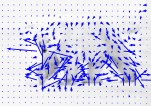
\includegraphics[width = 100pt]{Images/vector_fieldOurs.png}
\caption{Champs de vecteurs de l'image S}
      \end{minipage}\hfill
         \begin{minipage}{0.5\textwidth}
     \centering
     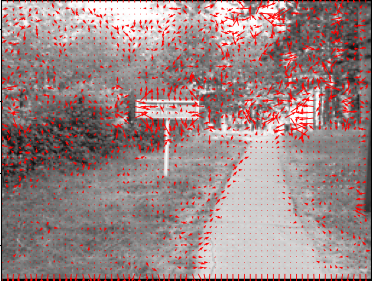
\includegraphics[width = 100pt]{Images/vector_fieldOursT.png}
\caption{Champs de vecteur de l'image T}
      \end{minipage}\hfill
      \end{figure}
Ces images représentent les champs de vecteurs dont le gradient de I devra se rapprocher le plus possible.
      \begin{figure}[!h]
        \begin{minipage}{0.5\textwidth}
     \centering
      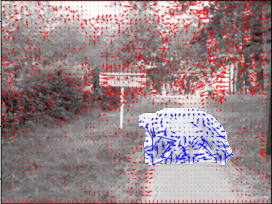
\includegraphics[scale=0.5]{Images/V.png}
      \caption{Nouveau domaine}
      \end{minipage}\hfill
              \begin{minipage}{0.5\textwidth}
     \centering
      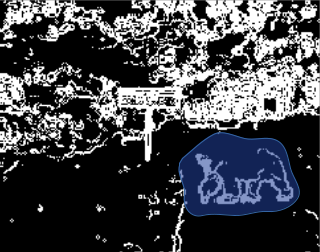
\includegraphics[scale=0.4]{Images/gradient.png}
      \caption{Nouveau domaine}
      \end{minipage}\hfill
      \end{figure}
Nous devons donc résoudre l'équation suivante : 
\begin{center}
$ \Delta I = div(V)$
\end{center}
Afin de pouvoir résoudre cette équation il faut imposer des conditions sur le bord. En appliquant l'effet miroir à l'image initiale alors, nous obtenons un signal symétrique et il est donc possible d'appliquer la transformée de Fourier pour résoudre le problème.  Les conditions imposées sont donc des conditions de Neumann.

Ainsi en calculant la transformée de Fourier du Laplacien nous obtenons : $\widehat{\Delta I} = \widehat{div(V)}$

\begin{equation}
\begin{aligned}
\left(\frac{2\pi i x}{M}\right)^2 \widehat{I}+\left(\frac{2\pi i y}{N}\right)^2 \widehat{I} & = \left(\frac{2\pi i x}{M}\right) \widehat{V_1}+\left(\frac{2\pi i y}{N}\right) \widehat{V_2}\\
\left(\left(\frac{2\pi i x}{M}\right)^2+\left(\frac{2\pi i y}{N}\right)^2\right) \widehat{I} & = \left(\frac{2\pi i x}{M}\right) \widehat{ V_1}+\left(\frac{2\pi i y}{N}\right) \widehat{V_2}\\
\end{aligned}
\end{equation}
\begin{equation}
\begin{aligned}
\widehat{I} = \frac{\left(\frac{2\pi i x}{M}\right) \widehat{ V_2}+\left(\frac{2\pi i y}{N}\right) \widehat{V_1}}{\left(\left(\frac{2\pi i x}{M}\right)^2+\left(\frac{2\pi i y}{N}\right)^2\right)}
\end{aligned}
\end{equation}
Afin de retrouver I, il suffit d'appliquer la transformée inverse, à l'équation ci-dessus.
Les résultats obtenus avec cette méthode seront présentés dans une prochaine section. 
\section{Optimisation}
\subsection{Méthode de Douglas \cite{Douglas}}
Nous avons vu deux manières de résoudre l'équation de Poisson avec conditions aux bords de Dirichlet. Nous allons maintenant présenter une troisième méthode  : \\
\begin{center}
Le méthode de Douglas
\end{center}
Soit $I$, l'image à retrouver : 
%%%%%%%%%%%%%%%%%%%%%%%%%%%%%%%%%%%%%%%%
\subsubsection{D'un problème avec contraintes...}
Remarquons que le problème initial est un problème d'optimisation avec contraintes. En effet, nous voulons minimiser $\int_\Omega ||\nabla I-\nabla S||^2$. Avec la contrainte suivante : $I = T$ en dehors du domaine. \\
Ce problème d'optimisation peut donc être résolu à l'aide de différents algorithmes, mais avant ça, transformons-le en un problème sans contraintes. 

\subsubsection{... À un problème sans contraintes}
En utilisant des fonctions de pénalisation nous remarquons aisément que ce problème peut être ramené à un problème sans contraintes. Réécrivons donc celui-ci 
\begin{equation*}
\begin{aligned}{}
    min \int_\Omega ||\nabla I - \nabla S||^2 + \mathbb{1} _{D \backslash \Omega } (I) \\
    \end{aligned}
\end{equation*}{}
avec 
\begin{equation*}
\mathbb{1}_{ D \backslash \Omega }(I) =
	\left\{
	\begin{aligned}{}
	0 \ si\  I \in T \backslash \Omega \\
	+ \infty \ sinon
    \end{aligned}
    \right.
\end{equation*}{}
Dans la suite nous noterons $K = T\backslash \Omega$. K représente donc l'ensemble des images dont les pixels situés en dehors du domaine$\Omega$, coïncident avec T.\\
\begin{figure}[!h]
\centering
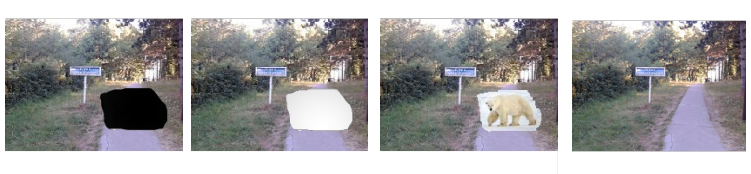
\includegraphics[scale=0.5]{Images/K.png}
\caption{Exemple d'images appartenant à K}
\end{figure}
\\
Nous avons bien équivalence entre notre problème sans contraintes et le problème (1). En effet, si I $\in K$, alors l'indicatrice vaut 0 et nous devons juste résoudre $min \int_\Omega ||\nabla I - \nabla S||^2 $. \\
Si au contraire $I \notin K$, alors nous devons minimiser quelque chose qui vaut plus $+\infty$. Le minimum n'existe pas, il n'y a pas de solutions.\\
 En effet, l'image I ne coïncide pas avec T à l'extérieur de $\Omega$,  la condition I = T en dehors du domaine n'étant pas respectée, le problème n'a pas de solution. \\
 Ce problème sans contraintes, traduit bien celui avec contraintes. Nous pouvons donc essayer de résoudre celui-ci, numériquement.\\ Afin d'être sûrs que le minimum existe, nous montrerons dans la suite que cette fonction est bien convexe. 
 Par commodité, nous noterons dans la suite : 
 \begin{equation*}
 \begin{aligned}
 F(I) &=   \int_\Omega ||\nabla I - \nabla S||^2 + \mathbb{1} _{T\backslash \Omega } (I) \\
 & = f(I)+ g(I)
 \end{aligned}
 \end{equation*}
\subsubsection{La convexité...}
Montrons que K est convexe. 
Soit u et v deux images appartenant à K, alors, les pixels de u et de v, se situant à l'extérieur de $\Omega$, coïncident avec les pixels de T. \\
Considérons maintenant une nouvelle image : 
\begin{center}
$M = \lambda u+(1-\lambda)v$
\end{center}
Les pixels de u et v coïncidant avec ceux de T à l'extérieur, nous pouvons réécrire les pixels de $M$ de la manière suivante. \\

\begin{equation*} 
M (i,j) = 
\left\{
\begin{aligned}
\lambda u(i,j) +(1-\lambda) v(i,j), \ \ (i,j) \in \Omega\\
\lambda T(i,j) +(1-\lambda )T(i,j))  \ \ (i,j)\notin \Omega
\end{aligned}
\right.
\end{equation*}
Ainsi, pour $(i,j) \notin \Omega$ : \\
\begin{center}
$M_{i,j} = \lambda T_{i,j}+(1-\lambda) T_{i,j} = T_{i,j}$
\end{center}
Ainsi, les pixels de M n'appartenant pas à $\Omega$, coïncident avec T. M appartient bien à K. Et K est donc convexe.\newline
K étant convexe, et non vide, (T en particulier appartient à K), alors la fonction $\mathbb{1}_K(I)$ est convexe. \newline
Enfin montrons la convexité de $||\nabla I-\nabla S||^2$.\newline
La norme étant une fonction convexe et croissante, alors la fonction : $||.||^2$ est elle aussi convexe. \\
Nous avons donc $f et g$, convexes, ainsi, la fonction $F =f+g$ est elle aussi convexe. Elle admet donc un minimum. Nous pouvons ainsi résoudre numériquement ce problème.
\subsubsection{... Pour utiliser l'algorithme de Douglas...}
L'algorithme que nous allons utiliser est l'algorithme de Douglas-Rachford. Cet algorithme permet d'approcher le minimum  d'une fonction $F = f+g$. \\
 $f$ et $g$ étant des fonctions convexes, comme montré dans la partie précédente, nous pouvons utiliser cet algorithme.
\paragraph{L'algorithme}
À chaque itération, sont calculés : 
\begin{center}
$x_{k+1} = prox_f(y_k)$\\
$y_{k+1} = y_k+prox_g(2x_{k+1}-y_k)-x_{k+1}$
\end{center}{}
Il est donc nécessaire de calculer les opérateurs proximaux respectifs de $f$ et $g$. 
\subsubsection{... Avec les opérateurs proximaux ...}
Un opérateur proximal est défini comme suit : 
\begin{center}
\begin{equation*}
\begin{aligned}
prox_f(x) = argmin_u \left\{ \frac{||u-x||^2}{2}+ f(u)\right\}
\end{aligned}
\end{equation*}
\end{center}
\cite{Opti}
\paragraph{Opérateur proximal de f}
\begin{equation*}
prox_f(x) = argmin_u\left\{\frac{||u-x||^2}{2}+||\nabla u -\nabla S ||^2 \right\}
\end{equation*}
Afin de faciliter les notations notons :
\begin{equation*}
h(u) = \frac{||u-x||^2}{2}+||\nabla u -\nabla S ||^2
\end{equation*} 
Nous cherchons donc 
\begin{center}
$argmin_u h(u)$
\end{center}
ie. u qui minimise la fonction h, autrement dit, un u qui annule le gradient de h.\\
En utilisant Taylor Young, 

\begin{equation*}
\begin{aligned}
h(u+k) -h(u) &= \frac{||u+k-x||^2}{2}+||\nabla  (u+k) -\nabla S ||^2- \frac{||u-x||^2}{2}-||\nabla u -\nabla S ||^2\\
& = \frac{||k||^2+2\left<u-x,k\right>}{2}+||\nabla k||^2+2\left<\nabla u-\nabla S, \nabla k\right>\\
& = O(||k||^2)+\left<u-x,k\right>-2\left<div(\nabla u-\nabla S), k\right>\\
& = \left<u-x-2div(\nabla u-\nabla S), k\right>\\
\end{aligned}
\end{equation*}
Nous obtenons le gradient de h.
\begin{equation*}
\begin{aligned}
\nabla h(u) &= u-x-2div(\nabla u - \nabla S)\\
& = u-x-2(\Delta u -\Delta S)
\end{aligned}
\end{equation*}
En résolvant $\nabla h(u) = 0$, nous pourrons trouver  : $prox_f(x) $. \\	
	\begin{equation*}
		\begin{aligned}
		\nabla h(u) &= 0\\
		u-x-2(\Delta u -\Delta S) & =0\\
		u-2\Delta u = x-2\Delta S
		\end{aligned}
\end{equation*}
Afin de trouver u, nous utiliserons la méthode des différences finies. En discrétisant le laplacien de u, comme nous l'avons vu dans la section (1) : 
\begin{equation*}
 -2u(x+1,y) -2 u(x-1,y)-2u(x,y+1) -2 u(x,y-1) +9\times u(x,y) =  y_k-  2\Delta S(x,y)
\end{equation*}
En mettant ce système sous forme matricielle nous pourrons approcher u en faisant une inversion matricielle. 
Nous pouvons donc numériquement approcher $prox_f(x)$.

\paragraph{Opérateur proximal de g}
g étant la fonction indicatrice suivante : 
\begin{equation*}
\mathbb{1}_{ D \backslash \Omega }(I) =
	\left\{
	\begin{aligned}{}
	0 \ si\  I \in T \backslash \Omega \\
	+ \infty \ sinon
    \end{aligned}
    \right.
\end{equation*}{}
Nous avons donc 
\begin{equation*}
prox_g(x) =  argmin_u\left\{\frac{||u-x||^2}{2}+ \mathbb{1}_K(u)\right\}
\end{equation*}
Nous savons que $prox_g(x)$ existe puisque la fonction g est convexe et la fonction norme est elle aussi convexe.\newline
Notons $h(u) = \frac{||u-x||^2}{2}+ \mathbb{1}_K(u)$ 
Comme nous l'avons vu cette fonction n'admet un minimum que si $u \in K$. Supposons donc $u \in K$.\\
 Alors chercher $argmin_u \left\{h(u)\right\}$ est équivalent à chercher $argmin_{u\in K} \left\{\frac{||u-x||^2}{2}\right\}$.\\
Il est donc évident que u= x, mais u $\in $ K. Ainsi : dans notre cas, $prox_g(x) = L$.
avec L une image appartenant à K, et dont les pixels à l'intérieur de $\Omega$ coïncident avec x.\\
\subsubsection{Convergence de l'algorithme vers la solution}
\begin{figure}[!htb]
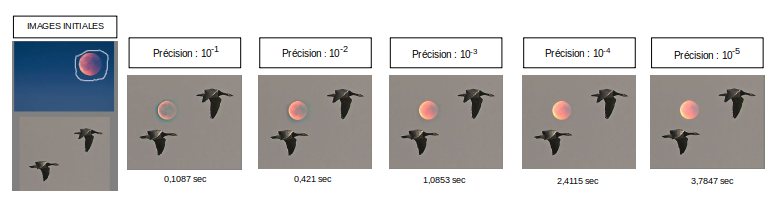
\includegraphics[scale=0.6]{Images/Resultats/conv1.png}
\caption{Convergence de l'algorithme vers la solution}
\end{figure}
\begin{figure}[!htb]
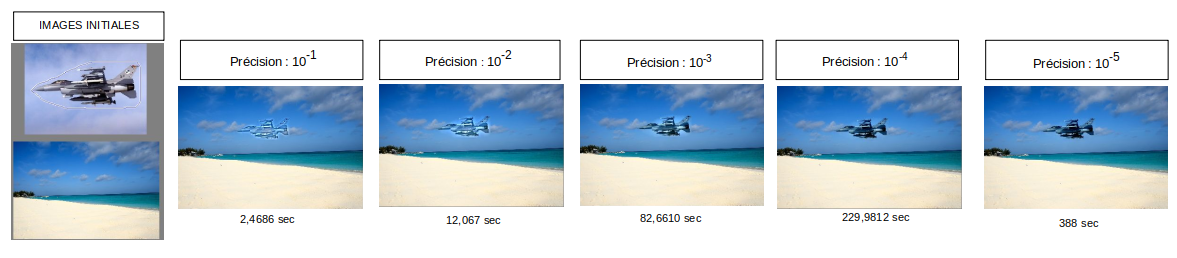
\includegraphics[scale=0.4]{Images/Resultats/conv2.png}
\caption{Convergence de l'algorithme vers la solution}
\end{figure}
L'algorithme de Douglas converge bien vers une solution I qui résout le problème initial.
\subsubsection{Temps et coût de l'algorithme}
L'algorithme semble être très efficace, malheureusement en termes de temps de calcul, il est très long. Nous ferons dans la prochaine partie un tableau comparatif des temps de calculs effectués sur des images de tailles différentes.\\
Nous avons considérablement amélioré  le temps de calcul de l'algorithme de Douglas-Rachford, en utilisant l'algorithme du gradient conjugué \cite{Gradient}, afin d'inverser la matrice de l'opérateur proximal de $f$. Malgré tout, l'algorithme est encore lent sur de grandes images. Nous choisissons une précision de $10^{-5}$, afin d'avoir des résultats comparables à ceux obtenus avec les méthodes précédentes sur toutes les images testées. Le nombre d'itérations de l'algorithme devient alors très important. Pour certaines images (voir ci-dessous) une précision de $10^{-3}$ de l'algorithme est suffisante pour obtenir des résultats convenables. Pour d'autres en revanche il faut augmenter cette précision(voir ci-dessus avec l'avion).\\
Nous avons amélioré les temps de calculs en appliquant une méthode de sur-relaxation sur l'algorithme de Douglas-Rachford, avec un $\rho  =1.85$. À chaque itération nous calculons donc :
\begin{center} 
\begin{itemize}
\item $x_{k+1} = prox_f(y_k)$
\item $y_{k+1} = y_k+\rho_k(prox_g(2x_{k+1}-y_k)-x_{k+1})$
\end{itemize}
\end{center}
($1<\rho<2$).\\
Cependant, le temps de calcul est encore élevé sur de grandes images.
Afin de réduire ce temps de calcul il faudrait donc que l'algorithme converge encore plus rapidement vers la solution. Pour cela, nous proposons d'augmenter l'ordre de discrétisation du Laplacien. Nous étions jusqu'à présent d'ordre 2, peut -être faudrait-il augmenter cette précision jusqu'à l'ordre 8.
\subsection{Tableau comparatif}
\begin{tabular}{|c|c|c|c|c|c|}
\hline
Taille de l'image S & Taille de l'image T& Temps Douglas & \shortstack{Temps Douglas \\(R)} &\shortstack{Temps différences\\ finies} & Temps Fourier\\
\hline
220 $\times$ 154 $\times$3 px & 304 $\times $252 $\times $3 px &  \shortstack{ 834 itérations\\ précision : 5$\times 10^{-5}$\\3.799 secondes} &\shortstack{ 547 itérations\\
précision : $5 \times 10^{-5}$\\ 2.2233 secondes}&  0.335 secondes & 0.355 secondes \\

\hline
304 $\times$ 252 $\times$3 px & 770$\times$844 $\times $3 px & \shortstack{ 1591 itérations\\ précision : 5$\times 10^{-5}$\\72.348 secondes} & \shortstack{ 1182 itérations\\
précision : $5 \times 10^{-5}$\\ 46.1067 secondes} & 0.797 secondes & 1.640 secondes \\
\hline
400 $\times$ 300 $\times$3 px & 1200$\times$800$\times $3 px & \shortstack{ 6224 itérations\\ précision : 5$\times 10^{-5}$\\440.886 secondes} &\shortstack{3884 itérations\\ précision : 5$\times 10^{-5}$\\205.8105 secondes} &1.05 secondes & 2.102 secondes \\
\hline
400 $\times$ 300 $\times$3 px & 614$\times$441$\times $3 px & \shortstack{ 5448 itérations\\ précision : 5$\times 10^{-5}$\\366.0.34 secondes}&\shortstack{4046 itérations\\ précision : 5$\times 10^{-5}$\\224.3881 secondes} & 0.877 secondes & 0.8576 secondes \\
\hline
220 $\times$ 154 $\times$3 px & 263$\times$192$\times $3 px & \shortstack{ 861 itérations\\ précision : 5$\times 10^{-5}$\\4.056 secondes} &\shortstack{510 itérations\\ précision : 5$\times 10^{-5}$\\2.3466 secondes}& 0.0892 secondes & 0.1754 secondes \\
\hline
\end{tabular}\\
\newline 
Temps Douglas (R) est la méthode de surrelaxation couplée à la méthode de Douglas, $\rho = 1.89$. Nous remarquons qu'à l'aide de cette méthode, nous pouvons considérablement diminuer le nombre d'itérations de l'algorithme de Douglas-Rachford et ainsi améliorer le temps de calcul de celui-ci. (jusqu'à t/2, sur de grandes images).\\
Les résultats que nous obtenons avec les différentes images sont très similaires à ceux obtenus avec les différences finies. Nous pouvons bien sûr raccourcir le temps de calcul de l'algorithme de Douglas-Rachford, en diminuant la précision. Mais dans ce cas, certains résultats sont moins convenables.
\section{Amélioration du collage}
Après avoir implémenté des "sliders", permettant de bouger la sélection sur l'image de fond, nous nous sommes compte que la sélection est parfois trop grande, et peut cacher des objets, ou choses importantes sur l'image de fond : 
\begin{figure}[!htb]
\centering
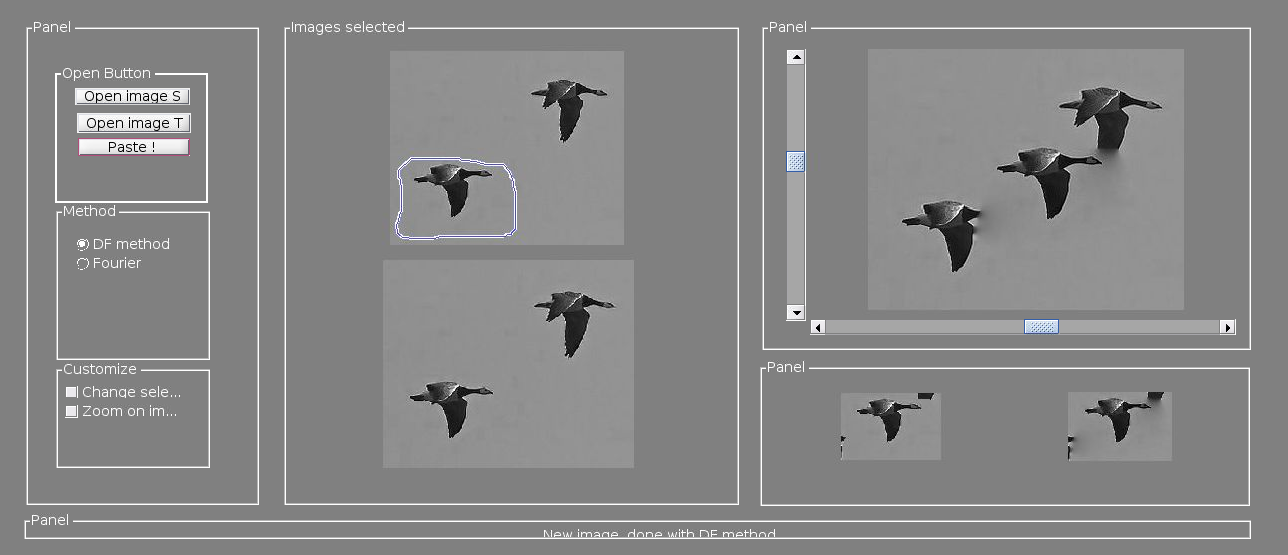
\includegraphics[scale=0.25]{Images/pb.png}
\caption{Problème rencontré}
\end{figure}
Nous voyons bien, ci-dessus, qu'en sélectionnant une grande zone autour de la lune dans l'image S,le collage cache effectivement l'oiseau, objet pourtant important de l'image T. Afin de résoudre ce problème, nous avons opté pour la comparaison des gradients dans chaque image. En effet, si le gradient de T est supérieur à celui de S, alors cela signifie que l'image T, possède un objet, ou un contour à cette position tandis que S ne possède rien d'important à la même position. Nous pouvons donc "réduire" la sélection et la modifier en ce pixel. Nous obtenons donc la figure suivante en utilisant cette propriété :
\begin{figure}[!h]
\centering
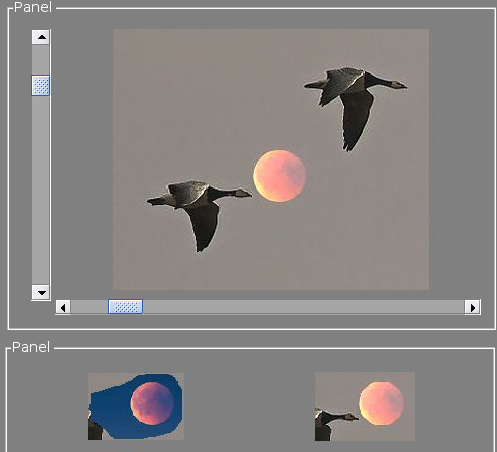
\includegraphics[scale=0.25]{Images/sol.png}
\caption{Problème résolu, algorithme utilisé : Différence Finie}
\end{figure}
\newpage
Cependant cette "amélioration" à ses limites, en effet, l'intérieur de la lune ne possède que très peu de variations et presque aucun contours, ainsi, si la lune se situait exactement sur la tête de l'oiseau, certains pixels à l'intérieur de celle-ci serait "supprimé" de la sélection, et ainsi, le résultat ne serait pas satisfaisant.

\section{Résultats obtenus}
\begin{figure}[!htb]
   \begin{minipage}{0.33\textwidth}
     \centering
     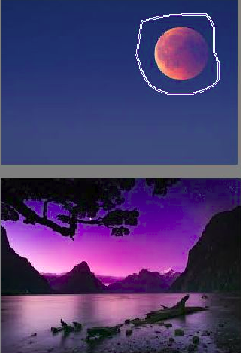
\includegraphics[width = 150pt]{Images/Resultats/LuneLand.png}
     \caption{Images sélectionnées}
      \end{minipage}\hfill
   \begin{minipage}{0.33\textwidth}
     \centering
     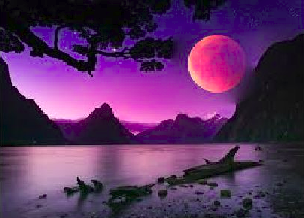
\includegraphics[width = 150pt]{Images/Resultats/LuneDF.png}
     \caption{Différences finies}
      \end{minipage}\hfill
   \begin{minipage}{0.33\textwidth}
     \centering
     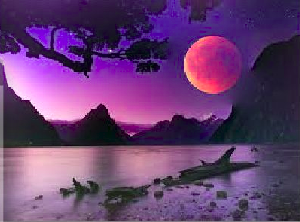
\includegraphics[width= 150pt]{Images/Resultats/LuneFourier.png}
     \caption{Fourier}
   \end{minipage}
\end{figure}

\begin{figure}[!h]
\centering
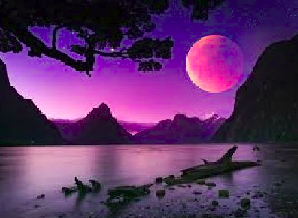
\includegraphics[scale=0.5]{Images/Resultats/LuneDFChangeSel.png}
\caption{Différence Finie ajustée}
\end{figure}

\begin{figure}[!htb]
   \begin{minipage}{0.33\textwidth}
     \centering
     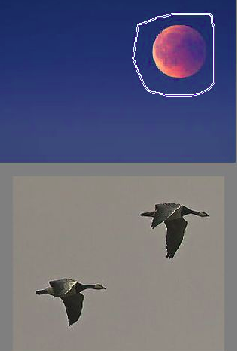
\includegraphics[width = 150pt]{Images/Resultats/LuneOiseau.png}
     \caption{Images sélectionnées}
      \end{minipage}\hfill
   \begin{minipage}{0.33\textwidth}
     \centering
     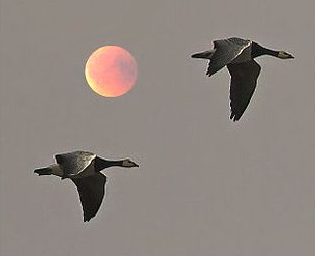
\includegraphics[width = 150pt]{Images/Resultats/LuneOiseauD.png}
     \caption{Différences finies}
      \end{minipage}\hfill
   \begin{minipage}{0.33\textwidth}
     \centering
     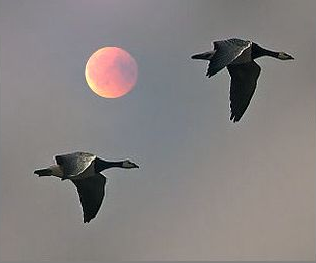
\includegraphics[width= 150pt]{Images/Resultats/LuneOiseauF.png}
     \caption{Fourier}
   \end{minipage}
\end{figure}


\begin{figure}[!htb]
   \begin{minipage}{0.33\textwidth}
     \centering
     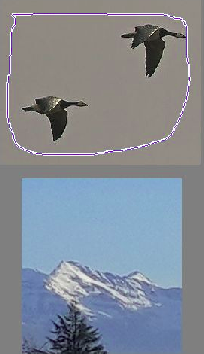
\includegraphics[width = 150pt]{Images/Resultats/OiseauMont.png}
     \caption{Images sélectionnées}
      \end{minipage}\hfill
   \begin{minipage}{0.33\textwidth}
     \centering
     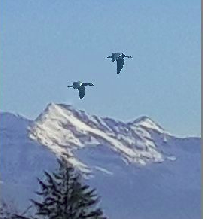
\includegraphics[width = 150pt]{Images/Resultats/oiseauRenduDF.png}
     \caption{Différences finies}
      \end{minipage}\hfill
   \begin{minipage}{0.33\textwidth}
     \centering
     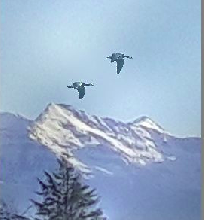
\includegraphics[width= 150pt]{Images/Resultats/OiseauRenduFourier.png}
     \caption{Fourier}
   \end{minipage}
\end{figure}

\begin{figure}[!h]
\centering
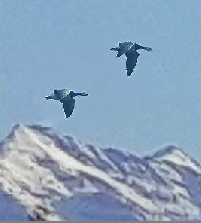
\includegraphics[scale=0.5]{Images/Resultats/zoomOiseauDF.png}
\caption{Différence Finie zoom}
\end{figure}

\begin{figure}[!htb]
   \begin{minipage}{0.33\textwidth}
     \centering
     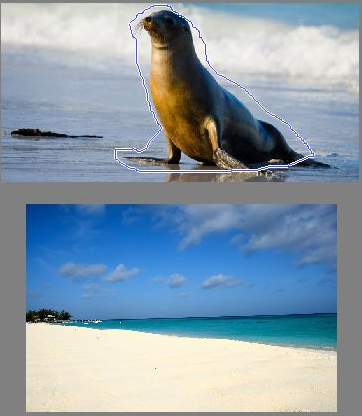
\includegraphics[width = 150pt]{Images/Resultats/otariePlage.png}
     \caption{Images sélectionnées}
      \end{minipage}\hfill
   \begin{minipage}{0.33\textwidth}
     \centering
     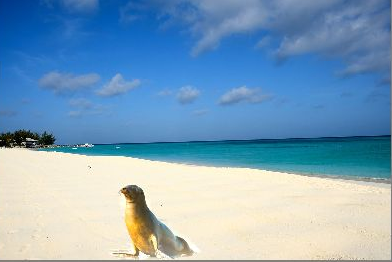
\includegraphics[width = 150pt]{Images/Resultats/OtariePlageD.png}
     \caption{Différences finies}
      \end{minipage}\hfill
   \begin{minipage}{0.33\textwidth}
     \centering
     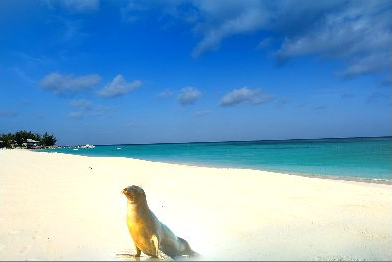
\includegraphics[width= 150pt]{Images/Resultats/OtariePlageF.png}
     \caption{Fourier}
   \end{minipage}
\end{figure}

\section{Comparaison}
\newpage
\subsection{Différences de résultat}
En comparant les images ci-dessus, nous pouvons observer quelques différences entre la méthode de Fourier et celle des Différences finies. En effet, la méthode des différences finies ne travaille que sur une partie de l'image, celle qui va être collée, afin de l'adapter au mieux à l'image de fond. Le reste de l'image n'est pas modifié et on retrouve exactement l'image initiale T en dehors du domaine. \\
La méthode de Fourier elle, modifie toute l'image, elle n'adapte pas seulement la partie à coller, mais c'est toute l'image qui est modifiée. Fourier effectue un "mélange" des deux images. \\
Plus la précision de l'algorithme de Douglas augmente, plus le résultat obtenu avec celui-ci est proche de celui obtenu avec les différences finies.
\subsection{Différence de temps}
La méthode des différences finies fait intervenir une inversion matricielle, qui si elle est grande, augmentera significativement le temps de calcul de l'algorithme. Cette méthode consiste en la résolution d'un système plus ou moins grand, qui peut parfois prendre du temps. \\
Sur de grandes sélections, la méthode de Fourier, semble plus rapide, il est facile de calculer le gradient de l'image, et la fft ("fast fourier transform") est plus rapide. Sur de grandes sélections c'est donc cette méthode qui serait à privilégier.\\
La méthode de Douglas, est beaucoup plus lente, à cause du coût de l'opérateur proximal de $f$, et du nombre d'itérations répétées.  

\section{Implémentation}
Voici une présentation de l'interface et ses fonctionnalités.

\subsection{Interface}
Voici comment se présente notre interface : 
\begin{figure}[!h]
    \centering
    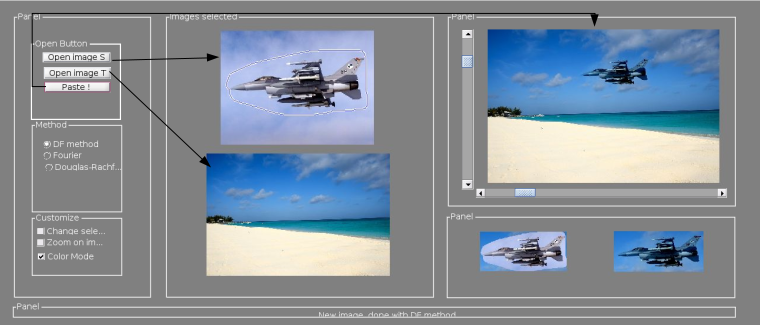
\includegraphics[scale = 0.3]{Images/interface.png}
    \caption{Interface 1.0}
\end{figure}{}
Elle est découpée en "blocs". Le premier bloc appelé "Open Button" se situe en haut à gauche, il permet l'ouverture d'images. En cliquant sur "Open Image S", une boite de dialogue s'ouvre et permet de charger une image présente dans l'ordinateur. De même en cliquant sur le bouton T. Une fois ces images chargées elles s'affichent dans le bloc numéro 2 appelé "Images selected". L'image la plus haute dans ce bloc correspond à l'image S, tandis que l'image si situant en bas affiche l'image T.
Il y a aussi un bouton "Save" permettant d'enregistrer l'image obtenue.\\ 
Une fois les images affichées, il faut sélectionner la région dite "à coller" dans l'image S, et la région où va se faire le collage dans l'image T.\\

\paragraph{Choix des méthodes}
Dans cette interface il est possible de sélectionner la méthode à utiliser. Le choix se porte sur 3 algorithmes : 
\begin{itemize}
    \item Les différences finies
    \item Fourier 
    \item Douglas-Rachford
\end{itemize}{}
Il suffit de sélectionner la méthode pour l'appliquer.
En cliquant sur le bouton "Paste !", présent dans le bloc "Open button", la nouvelle image est calculée et s'affiche dans le bloc "Main Result" situé en haut à droite. 
\paragraph{Les options}
D'autres options ont été ajoutées dans cette interface. Il est possible d'effectuer l'amélioration vue plus haut, en la sélectionnant, la case : "Change selection". Il est aussi possible de zoomer sur les différentes images, à l'aide de la case zoom. Enfin il est possible de travailler sur des images en couleur, en cochant la case adéquate(Si cette case n'est pas cochée, le résultat est affiché en niveau de gris). Toutes ces options se trouvent dans le bloc : Customizer.
\paragraph{Sliders}
Des sliders sont situés de parts et d'autres de l'image finale, dans le bloc "main result". En activant ces sliders, il est donc possible de bouger la sélection à l'intérieur de l'image. Ainsi l'image finale est recalculée, et l'image à coller sera collée à la position indiquée par les sliders.
\paragraph{bloc Results}
Le dernier bloc est un bloc d'affichage, il affiche, une fois créée, l'image obtenue par l'algorithme sélectionné, dans le bloc correspondant. Cela permet une comparaison rapide.
\subsection{Organisation du code}
Nous avons organisé le code sous forme de classes. Le projet contient 4 classes principales, la classe, Fourier, la classe DFinies, la classe Douglas et enfin la classe  Mask. Notre projet contient aussi deux fonctions, la fonction copier/coller et la fonction du gradient conjugué.

%%%%%%%%%%%%%%%%%%%%%%%%%%%%%%%%%%%%%%%%%%%%%%%%%%%

\begin{figure}[!h]
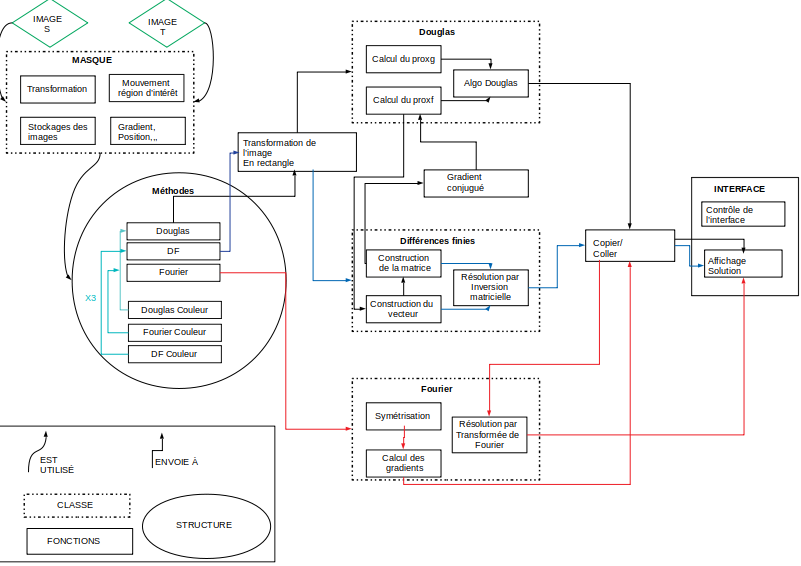
\includegraphics[scale=0.65]{Images/code/schema.png}
\caption{Structure et interactions du code}
\end{figure}
\newpage

\paragraph{Explication du schéma}
Le code est organisé en différentes classes (4).
\paragraph{Douglas}
Cet algorithme étant plutôt long (en terme de temps), nous ne travaillerons pas sur l'image entière mais sur le plus petit rectangle autour de la sélection. En d'autres termes nous collerons l'image S sur une sous-image de T, que nous réinsérerons par la suite au bon endroit dans T. Afin de résoudre le problème à l'aide de l'algorithme de Douglas, nous avons crée une classe du même nom.  A l'intérieur de celle-ci, nous calculons les opérateurs proximaux nécessaires. Avec une particularité, l'opérateur proximal de la norme nécessite la construction d'une matrice. Afin d'éviter les doublons nous utilisons donc la classe FDSystem, pour calculer cette matrice, et le vecteur associé. Puis nous inversons le système à l'aide de l'algorithme du gradient conjugué. 
\paragraph{Différences finies}
Pour résoudre le problème avec les différences finies, la classe DFSystem, nous permet de calculer la matrice A, le vecteur b et enfin d'inverser le système pour trouver la solution. De la même manière que pour Douglas, nous ne travaillons pas sur l'image entière mais sur une sous-image que nous recollons au bon endroit à la fin.
\paragraph{Fourier}
Dans la classe Fourier nous symétrisons les images, puis calculons les gradients de celles-ci. Les images représentant les gradients sont par la suite fusionnées avant d'être envoyées à la fonction de résolution de la classe Fourier. 
\paragraph{Mask}
La classe Mask, permet le traitement d'images et de masque, elle est mise à jour pendant tout le programme. C'est notamment elle qui permet le découpage d'image, la fusion de deux images, le redimensionnement des masques si besoin. 
\paragraph{La fonction gradient conjugué}
Elle permet de trouver la solution au système Ax=b de manière rapide.
\paragraph{La fonction copier coller} 
Elle écrase certains pixels d'une image par les pixels d'une autre.
\section{Conclusion}
L'équation de Poisson avec conditions aux bords de Dirichlet permet donc l'insertion d'une image dans une autre. A l'inverse, nous pouvons utiliser cette équations pour effacer certaines parties d'une image, ou encore pour augmenter la luminosité d'une image. Cette méthode est plutôt efficace même si elle possède ses limites.En effet, la couleur de l'objet à coller est par conséquent bien modifiée, qui parfois rends le collage beaucoup moins naturel. De même une grande sélection, est visible sur un fond très détaillé. Plus l'image de fond 'T' possède des variations, contours, détails, plus le collage devient mauvais. \\
Nous avons précédemment vu qu'une sélection plutôt large pouvait masquer des objets importants de l'image T. Ce problème peut être en partie résolu par des systèmes de comparaisons de gradients ou de moyenne mais le résultat n'est pas pas fiable, surtout si l'image à coller possède peu de variations. Cependant nous pouvons essayer d'étendre la résolution de cette équation sur des vidéos, en voulant incruster une vidéo dans une autre. Par exemple, réussir à incruster un vol d'oiseaux dans une vidéo. Si le vol se déplace dans la vidéo il faudrait être capable de détecter les mouvements de l'oiseau, (à l'aide de carte de disparité) afin de déplacer la sélection en même temps que l'objet.
\cite{Image}
\cite{Douglas}
\cite{Gradient}
\cite{Opti}
\cite{Fourier}
\bibliographystyle{plain}
\bibliography{references}
\end{document}
